
% Szkielet dla pracy inżynierskiej pisanej w języku polskim.

\documentclass[polish,bachelor,a4paper,11pt,twoside]{ppfcmthesis}

\usepackage[utf8]{inputenc}
\usepackage[OT4]{fontenc}
\usepackage{eurosym}
\usepackage{latexsym}
\usepackage{rotating}
\usepackage{hyperref}
\usepackage[font=small,labelsep=period]{caption}

\usepackage[all]{nowidow}

\usepackage{enumitem}
\setlist[enumerate]{itemsep=0mm}
\setlist[itemize]{itemsep=0mm}


\DeclareUnicodeCharacter{00A0}{~}

% Authors of the thesis here. Separate them with \and
\author{
   Mikołaj Błajek \album{99409} \and 
   Filip Rachwalak \album{99523} \and 
   Michał Słomkowski \album{100489}
}
\authortitle{}                                        % Do not change.
\title{Sterownik matrycy świetlnej w~oparciu o~mikrokontroler AVR}                   % Note how we protect the final title phrase from breaking
\ppsupervisor{dr~inż.~Roman Mielcarek} % Your supervisor comes here.
\ppyear{2014}                                         % Year of final submission (not graduation!)

\newcommand{\todo}[1]{}
\renewcommand{\todo}[1]{{\color{red} TODO: {#1}}}

\addto\captionspolish{\renewcommand{\figurename}{Rys.}}

\linespread{1.3}

\brokenpenalty10000\relax

\begin{document}

% Front matter starts here
\frontmatter\pagestyle{empty}%
\maketitle\cleardoublepage%

% Blank info page for "karta dyplomowa"
\thispagestyle{empty}\vspace*{\fill}%
\begin{center}Tutaj przychodzi karta pracy dyplomowej;\\oryginał wstawiamy do wersji dla archiwum PP, w pozostałych kopiach wstawiamy ksero.\end{center}%
\vfill\cleardoublepage%

% Table of contents.
\pagenumbering{Roman}\pagestyle{ppfcmthesis}%
\tableofcontents* \cleardoublepage%

% Main content of your thesis starts here.
\mainmatter%
\chapter{Wstęp}

\section{Wprowadzenie}

W ostatnich kilkudziesięciu latach ilość informacji, z~jaką styka się człowiek w~ciągu swojego życia, wzrosła wielokrotnie. Zjawisko to nie miało miejsca nigdy wcześniej w~historii ludzkości. W~związku w~wszechobecnością wszelkiego typu treści ludzie wypracowali sobie odruchy podświadomego filtrowania informacji, które z~ich punktu widzenia są niepotrzebne lub nieinteresujące. Stawia to przed twórcami zajmującymi się wizualizacją nowe wyzwania polegające na zwróceniu uwagi potencjalnego odbiorcy i~prezentacji informacji w~szybki, prosty i~atrakcyjny sposób. Ma to szczególne znaczenie w~wymiarze komercyjnym, gdzie od skuteczności reklamy w~dużej mierze zależy powodzenie przedsiębiorstwa.

Tablice informacyjne i~reklamowe oparte o~wyświetlacze LED są zauważalne z~powodu dobrej widoczności zarówno w~dzień, jak i~w~nocy oraz prezentacji obrazów ruchomych, co naturalnie przyciąga wzrok odbiorcy.

Zapoznając się z~istniejącymi urządzeniami tego typu zauważa się archaiczność stosowanych w~nich rozwiązań technicznych, takich jak użycie interfejsów szeregowych w~standardzie RS232 i~braku łatwych w~obsłudze programów do tworzenia animacji. Często producenci nie udostępniają takiego programu użytkownikom, oferując w~zamian usługę tworzenia animacji, co generuje dodatkowe koszty dla właściciela urządzenia.

Opracowano więc projekt tablicy świetlnej, która posiada złącze USB do komunikacji z~komputerem PC oraz przechowuje dane na powszechnie stosowanej karcie pamięci typu SD.~Urządzenie, widoczne na rysunku \ref{zdj-calosc}, ma budowę modułową, co przy pewnych modyfikacjach oprogramowania umożliwia zmianę rozmiaru tablicy z~domyślnych ośmiu paneli do mniejszej ich liczby lub też ustawienie w~dwa rzędy (konfiguracja $4 \times 2$).

\begin{figure}[htb]
	\begin{center}
		\includegraphics[width=\textwidth]{figures/overall.jpg}
	\end{center}
	\caption{Widok ogólny urządzenia.}
	\label{zdj-calosc}
\end{figure}

Celem pracy jest zaprojektowanie i~wykonanie sterownika diodowej matrycy świetlnej wraz z~oprogramowaniem dla komputera PC umożliwiającym tworzenie animacji tekstowych i~graficznych możliwych do wyświetlenia na skonstruowanym urządzeniu.

\section{Struktura pracy}

Niniejsza praca składa się pięciu rozdziałów oraz dodatku. Rozdział \textit{Podstawy teoretyczne} omawia w~ogólny sposób najważniejsze zagadnienia związane z~projektem, jak idea wyświetlania multipleksowego na matrycach LED, opis mikrokontrolera AT90USB647, interfejsu USB i~kart pamięci SD oraz podstawowe informacje na temat fontów komputerowych.

Rozdział trzeci zawiera zarys projektu systemu oraz opis formatów plików służących do wymiany informacji między urządzeniem a~komputerem. Rozdział czwarty szczegółowo opisuje wykonanie systemu na trzech obszarach: urządzenia elektronicznego, oprogramowania mikrokontrolera oraz programu na komputer PC.~Rozdział piąty stanowi podsumowanie pracy.  W~dodatkach zamieszczono: instrukcje obsługi dla użytkowników omawiające sposób nawigacji po menu tablicy i~tworzenie animacji w~programie komputerowym, parametry zasilacza sieciowego oraz spis zawartości dołączonej płyty CD.

Niniejszą pracę realizowało trzech niżej wymienionych autorów. Sekcje poświęcone danemu zagadnieniu są autorstwa osoby, która zajmowała się nim przy projektowaniu i~wykonywaniu urządzenia. Poniżej przedstawiono podział zadań.

\textbf{Mikołaj Błajek} opracował obsługiwany przez urządzenie format plików M2F oraz zaimplementował jego odtwarzanie na komputerze PC oraz na sterowniku. Zaimplementował takie elementy funkcjonalności tablicy, jak menu, zegar wraz z~jego ustawianiem oraz wybór i~wczytywanie plików animacji. Zaprojektował dwa fonty, dostosowując je do określonych wymagań.~Poza tym wykonał drobne prace montażowe.

\textbf{Filip Rachwalak} opracował format plików MMF, zaprojektował i~zaimplementował aplikację do tworzenia animacji na komputerze PC, w~szczególności, zaprojektował metody rysowania wewnątrz obszarów (\textit{obszar} --- patrz \ref{slownik}) jak i~samych obszarów i~dodawania efektów tekstowych. Zaimplementował również generator plików wyjściowych animacji. Dokonał montażu całego urządzenia z~dostarczonych płytek drukowanych i~elementów elektronicznych.

\textbf{Michał Słomkowski} w~ramach niniejszej pracy zaprojektował urządzenie od strony sprzętowej, w~szczególności: opracował schemat ideowy modułu sterownika wraz z~projektem ścieżek płytki drukowanej oraz zaprogramował elementy oprogramowania mikrokontrolera na niskim poziomie abstrakcji, jak obsługa przerwań, portów wejścia-wyjścia, czasomierzy, zintegrował używane biblioteki obsługi kart SD, magistrali USB oraz systemu plików FAT.~Dokonał również montażu sterownika.

\section{Słownik pojęć}
\label{slownik}

W celu uniknięcia niejednoznaczności podczas czytania niniejszej pracy, poniżej opisano stosowane w~niej terminy.

\begin{itemize}
	\item \textit{Animacja} --- pełna sekwencja klatek (\textit{klatka} --- patrz niżej) odtwarzana przez mikrokontroler na tablicy. Jest wizualizacją wygenerowanego przez aplikację pliku,

	\item \textit{driver} --- płytka drukowana, na której znajdują się wzmacniacze mocy sterujące wyświetlaczami,

	\item \textit{efekt} --- pojedyncza czynność modyfikująca tekst lub grafikę w~obrębie \textit{obszaru} np. \textit{Przewijanie w~lewo}, wyrównanie tekstu \textit{Do środka} lub \textit{Negatyw},
	
	\item \textit{font} --- zestaw znaków drukarskich o~wspólnych cechach \cite{fonts},

	\item \textit{ekran} --- odwzorowanie powierzchni tablicy w~graficznym interfejsie użytkownika, widoczne w~jego głównej części. Wymiary ekranu odpowiadają faktycznym wymiarom tablicy ($128 \times 16$ elementów świecących),
	
	\item \textit{font} --- oznaczają zestaw znaków pisarskich, opisujących kształt i wielkość liter, czcionka,
	
	\item \textit{klatka} --- pojedynczy stan ekranu. Animacja składa się z~następujących po sobie klatek,

	\item \textit{magistrala} --- zestaw szyn i~linii sygnałowych pomiędzy sterownikiem a~drajwerem, znajdujących się na płytce drukowanej magistrali,

	\item \textit{matryca} --- płytka drukowana grupująca cztery wyświetlacze $8 \times 8 $ w~jeden o~wymiarach $16 \times 16$. Jest połączona z~płytką drajwera,

	\item \textit{obszar} --- powierzchnia w~kształcie prostokąta rysowana przez użytkownika na ekranie za pomocą myszki. Użytkownik definiuje wyświetlaną treść w~obrębie zaznaczonej powierzchni,

	\item \textit{piksel} --- pojedyncza ,,dioda'' tablicy i~jej odwzorowanie na ekranie w~postaci białego pojedynczego kwadratu,

	\item \textit{plik animacji} --- plik o~rozszerzeniu \texttt{.m2f} wygenerowany przez aplikację, który zawiera pełną animację,

	\item \textit{projekt} --- 1. efekt pracy użytkownika: rozmieszczone na ekranie i~wyspecyfikowane obszary. Projekt można zapisać jako plik z~rozszerzeniem \texttt{.mmf} i~otworzyć go później. 2. całokształt pracy wykonanej przez autorów,

	\item \textit{sterownik} --- płytka drukowana zawierająca mikrokontroler AVR, sterująca zestawami,

	\item \textit{tablica} --- całe urządzenie, wszystkie moduły połączone w~całość,

	\item \textit{typografia} --- dziedzina wiedzy o zasadach składu drukarskiego, sposób prezentacji tekstu w sposób czytelny i estetyczny \cite{fonts},

	\item \textit{zestaw} --- połączone ze sobą płytki: matrycy, drajwera i~magistrali.
\end{itemize}

\chapter{Podstawy teoretyczne}

Niniejszy rozdział podsumowuje stan wiedzy na temat technologii wykorzystywanych przy konstrukcji tablicy. Omawia takie zagadnienia jak wyświetlacze matrycowe LED i~sposób ich sterowania, interfejs komunikacyjny USB i~karty pamięci typu SD.~Zamieszczono również podstawowe informacje na temat typografii z~racji wykorzystywania w~projekcie samodzielnie tworzonych fontów. Dołączono również spis używanych narzędzi programistycznych.

\section{Wyświetlacz matrycowy LED i~sterowanie multipleksowe}

\textit{Light-emitting diode}, dioda elektroluminescencyjna jest półprzewodnikowym elementem elektronicznym emitującym światło na skutek przepływającego przez nią prądu. Pod względem elektrycznym element ten zachowuje się jak zwykła dioda, pozwalając na przepływ prądu tylko, gdy jest on zgodny z~kierunkiem przewodzenia diody oraz gdy spadek napięcia na niej przekracza barierę potencjału złącza p-n, której wartość zależy od rodzaju zastosowanego półprzewodnika. 

Zasadniczym elementem tablicy świetlnej są wyświetlacze LED typu \mbox{JZM23882ASR} o~wymiarach zewnętrznych $53 \times 53$ mm, posiadające 64 diody LED koloru czerwonego zorganizowane w~matrycę o~wymiarach $8 \times 8$. Natężenie prądu przepływającego przez diodę może sięgać $30$ mA; w~projekcie, kierując się kompromisem między jasnością i~niezawodnością, ustalono prąd na $18$ mA.

\begin{figure}[t]
    \begin{center}
       \includegraphics[width=0.8\textwidth]{figures/ledmatrix.pdf}
    \end{center}

    \caption{Schemat ideowy wyświetlacza matrycowego LED typu \mbox{JZM23882ASR-GW}. Źródło \cite{ds-wysw}.}
    \label{schemat-wysw}
\end{figure}

Sterowanie każdą komórką wyświetlacza niezależnie w~tradycyjny sposób wymagałoby $ 8 \times 8 + 1 = 65 $ wyprowadzeń (64 katody i~jedna wspólna anoda). By ilość tą zmniejszyć, producent zastosował odmienny sposób sterowania: komórki umieszczone są w~węzłach siatki utworzonej z~przecinających się linii anod i~katod, co pokazane jest na rysunku \ref{schemat-wysw}.

Sterowanie multipleksowe wyświetlacza jest rodzajem sterowania dynamicznego, to znaczy, że w~celu uzyskania stabilnego obrazu należy z~odpowiednio dużą szybkością wysterowywać pojedynczą kolumnę lub wiersz, odczekać pewien czas a~następnie wysterowywać kolumnę lub wiersz następny. W~danej chwili aktywny jest tylko jeden wiersz/kolumna.

Wrażenie stabilnego obrazu powstaje dzięki bezwładności oka ludzkiego, które uśrednia szybko zmieniające się obrazy. Zakładając, że wyświetlacz ma osiem kolumn, obserwator odbiera wrażenie świecenia wiersza z~jedną ósmą swej maksymalnej jasności (zakładając liniowość percepcji oka). Praktyka pokazuje, że stabilny obraz uzyskuje się, gdy częstotliwość odświeżenia całego ekranu przekracza $250$ Hz \cite{sztuka2}.

W prezentowanym urządzeniu przełączanie aktywnej kolumny odbywa się co $200$ $\mu$s, co oznacza, że przerysowywanie ekranu odbywa się z~częstotliwością $312$ Hz.

\section{Mikrokontroler AVR typu AT90USB647}

\textit{AVR} to rodzina ośmiobitowych mikrokontrolerów jednoukładowych stworzona przez firmę Atmel. Została opracowana zgodnie z~założeniami zmodyfikowanej architektury harwardzkiej (rozdzielone pamięci danych i~programu, lecz wspólne szyny danych i~adresowa). W~pojedynczym układzie scalonym umieszczono, obok procesora, większość modułów niezbędnych do działania systemu mikroprocesorowego takich jak pamięć operacyjna, pamięć programu FLASH, timery systemowe, obwody wejścia/wyjścia itd. Fakt ten umożliwia budowanie urządzeń znacznie mniejszych i~pobierających mniej energii, niż porównywalne systemy złożone z~wielu układów scalonych.

Mikrokontroler jednoukładowy AT90USB647 jest przedstawicielem rodziny AVR, zastosowanym ze względu na zintegrowany sprzętowy interfejs USB strony urządzenia. Umożliwiło to łatwą implementację komunikacji tablicy świetlnej z~komputerem PC.~Poniżej omówiono pozostałe właściwości i~moduły mikrokontrolera, które wykorzystywane były w~konstrukcji tablicy, opracowane na podstawie noty katalogowej \cite{ds-avr}. Schemat blokowy przedstawiono na rysunku \ref{blokowy-avr}.

\begin{figure}[t]
    \begin{center}
       \includegraphics[width=\textwidth]{figures/avrdiagram.pdf}
    \end{center}

    \caption{Schemat blokowy mikrokontrolera AT90USB647. Źródło: \cite{ds-avr}.}
    \label{blokowy-avr}
\end{figure}

\begin{itemize}

\item Architektura typu RISC: 135 instrukcji, z~czego większość wykonywana w~jednym cyklu zegara, 32 rejestry ogólnego przeznaczenia, zegar do $16$ MHz,

\item $64$ kB pamięci FLASH przeznaczonej na kod wykonywalny,

\item $4$ kB pamięci operacyjnej RAM,

\item interfejs diagnostyczny JTAG (niewykorzystywany),

\item wbudowany interfejs USB 2.0 \textit{full-speed} i~\textit{low-speed} typu \textit{device} lub \textit{On-The-Go}, wykorzystywany tryb urządzenia i~transfery masowe dla klasy \textit{Mass Storage},

\item dwa przerwania zewnętrzne, dwa przerwania reagujące na zbocze konfigurowalne na wielu wyprowadzeniach,

\item dwa zegary/liczniki 16-bitowe pozwalające na zliczanie impulsów z~zegara taktującego lub zewnętrznego źródła z~zastosowaniem lub nie dzielnika częstotliwości, generujące przerwania przy przepełnieniu lub osiągnięciu wartości przechowywanej w~rejestrach porównujących. Wykorzystywane do generowania przerwań obsługujących wyświetlacz matrycowy, gwarantujące odświeżanie w~deterministycznym czasie,

\item licznik czasu rzeczywistego (RTC) z~zewnętrznym oscylatorem niezależnym od zegara głównego, niezbędny do implementacji zegara czasu urzędowego z~kalendarzem, generujący przerwania co sekundę, również w~trybach obniżonego poboru mocy,

\item interfejs SPI wspierający tryb \textit{master} i~\textit{slave} --- używany do komunikacji z~kartą SD oraz szeregowego programowania mikrokontrolera przez złącze ISP,

\item pozostałe, niewykorzystywane podsystemy (większość z~nich może generować przerwania): sześć kanałów PWM, komparator analogowy, interfejs $I^{2}C$, uniwersalny interfejs szeregowy (min.~RS232C), 10-bitowy przetwornik analogowo-cyfrowy, dwa timery/liczniki ośmiobitowe,

\item obwody odpowiadające za reset mikrokontrolera i~kontrolę napięcia zasilania (\mbox{\textit{Brown-Out}}),

\item \textit{watchdog} --- podsystem resetujący mikrokontroler w~przypadku, gdy mikrokontroler wpadnie w~martwą pętlę, co skutkuje zawieszeniem wykonywania się programu, 

\item wewnętrzny oscylator RC i~oscylator kwarcowy,

\item tryby obniżonego poboru mocy: \textit{Idle, ADC Noise Reduction, \mbox{Power-save}, \mbox{Power-down}, Standby} i~\textit{Extended Standby}.

\end{itemize}


\section{Magistrala USB i~klasa pamięci masowej}

USB (ang. \textit{Universal Serial Bus}) to standard definiujący warstwę fizyczną i~programową interfejsu łączącego różne urządzenia peryferyjne z~komputerem PC. W~chwili pisania niniejszej pracy aktualną jest wersja standardu 3.0. Dokument ten definiuje sposoby połączeń, kształty gniazd i~wtyków, sposoby implementacji modułów po stronie hosta (komputer PC) i~samych urządzeń oraz reprezentację ich w~systemach operacyjnych.

Magistrala USB ma topologię drzewa. Wszystkie urządzenia połączone są z~\textit{hostem} przy pomocy \textit{hubów}. Na samym szczycie znajduje się hub główny. Możliwe jest podłączenie do 127 urządzeń.~Szybkość przesyłu danych może wynosić od 1.5, 12, 480 MBit/s lub 5 GBit/s dla standardu 3.0. Urządzenia posiadają od jednego do kilku tzw. punktów końcowych (ang.  \textit{endpoint}). Między punktami końcowymi urządzenia i~hosta może być zestawiony wirtualny kanał komunikacyjny, w~którym płyną dane do i~z~urządzenia. Fizycznie przewód USB ma cztery linie: masę, zasilanie $+5$ V $500$ mA i~sygnałowe: D+, D-. Linie sygnałowe pracują różnicowo przy poziomach logicznych 0~V i~3,3~V.

Mając na uwadze uniwersalność magistrali standard definiuje cztery rodzaje połączeń (transferów) między punktami końcowymi: kontrolny, przerwaniowy, masowy i~izochroniczny. Każde urządzenie musi udostępniać co najmniej jeden kontrolny punkt końcowy. Transfer ten charakteryzuje się małą ilością danych w~ramce i~kontrolą poprawności. Jak wskazuje nazwa, służy on do kontroli pracy urządzenia i~ustalania jego konfiguracji. Transfer przerwaniowy posiada podobną charakterystykę do kontrolnego. Służy on do przesyłania małych porcji danych w~gwarantowanym czasie. Klasycznym zastosowaniem jest myszka komputerowa, gdzie przekazywanie bieżącej pozycji jest szczególnie istotne dla komfortu użytkownika (szczególnie w~grach).

Transfery masowy i~izochroniczny służą do przesyłu dużych ilości danych. Transfer izochroniczny wymusza dodatkowo natychmiastowość ich dostarczenia kosztem kontroli poprawności. Źle dostarczone są bezpowrotnie tracone. Istotne jest to w~zastosowaniach audio. Pojedyncze przekłamanie jest z~reguły praktycznie niesłyszalne, natomiast konieczność ponownego transferu pakietu danych spowodowałaby chwilową przerwę w~odtwarzaniu dźwięku. Dla transferu masowego priorytetem jest poprawność. Używają go wszystkie urządzenia pamięci masowej: \textit{pendrive}, dyski itd. Opisywana tablica korzysta głównie z~transferów masowych, z~racji wykorzystywanej klasy urządzenia \textit{Mass Storage}.

By przyporządkować podobne urządzenia wielu producentów do jednej grupy standard definiuje wiele \textit{klas}. Najważniejsze z~nich to: drukarka, pamięć masowa, hub, urządzenie komunikacji z~użytkownikiem (ang. \textit{Human Interface Device}), do której należą na przykład myszki i~klawiatury. Oprócz klasy, każde urządzenie posiada parę dwóch liczb identyfikatora producenta (\textit{Vendor ID}) i~produktu (\textit{Product ID}). Kod producenta przydzielany jest przez organizację \textit{usb.org}, twórców standardu.

\textbf{Klasa pamięci masowej} została zastosowana do implementacji komunikacji tablicy z~komputerem PC, dzięki czemu obecna w~urządzeniu karta SD widoczna jest w~systemie operacyjnym jako dysk twardy, niewymagający dodatkowych sterowników. Rozwiązanie takie podyktowane zostało prostotą obsługi przez użytkownika oraz istnieniem gotowych bibliotek implementujących wyżej wymienioną funkcjonalność, będących częścią pakietu \textit{LUFA}.

Protokół komunikacji w~omawianej klasie nie jest zależny od systemu plików i~działa na jednostkach danych --- blokach, których rozmiar jest charakterystyczny dla urządzenia, lecz zwykle wynosi 64 bajty. Na komunikację składają się trzy fazy \cite{interfejsy}:

\begin{enumerate}
\item wysłanie do urządzenia rozkazu,
\item odebranie statusu wykonania rozkazu,
\item odebranie danych, jeżeli zażądano odczytu.
\end{enumerate}

Pojedyncze urządzenie pamięci masowej może definiować wiele logicznych urządzeń LUN (ang. \textit{Logical UNit}), do których kierowane są polecenia. Bloki poleceń zawierają rozkazy zgodne z~tradycyjnymi interfejsami, jak ATA/ATAPI lub SCSI, co upraszcza implementację zarówno po stronie urządzenia, jak i~hosta. Oprócz nich stosowane są rozkazy dodatkowe, jak zerowanie urządzenia, przeładowanie buforów danych, sprawdzanie statusu itd.


\section{Karta SD}

\textit{Secure Digital} jest rodziną standardów przenośnych kart pamięci FLASH wywodzącą się z~wcześniejszego rozwiązania --- MMC, stosowaną w~wielu urządzeniach mobilnych, np. aparatach cyfrowych. Karta SD ma 9 wyprowadzeń i~wymiary $24 \times 32 \times 2.1$ mm. Na dzień pisania niniejszej pracy istnieją następujące wersje według pojemności:
\begin{itemize}
	\item SD --- pojemność do 4 GB,
	\item SDHC --- do 32 GB,
	\item SDXC --- do 2 TB pojemności
\end{itemize}
oraz rozmiaru:
\begin{itemize}
	\item Standard --- $ 24 \times 32 \times 2.1 $ mm,
	\item Mini --- $ 21.5 \times 20.0 \times 1.4 $ mm,
	\item Micro --- $ 15.0 \times 11.0 \times 1.0 $ mm.
\end{itemize}

Karta SD może komunikować się z~urządzeniem w~dwóch trybach: \textit{SD bus} oraz \textit{SPI bus}. SD bus jest własnościowym protokołem, co znaczy, że wymagana jest licencja na jego użycie. Tylko on pozwala na osiągnięcie pełnej szybkości transferu danych. Oprócz niego karty w~rozmiarze \textit{standard} implementują protokół zgodny z~interfejsem SPI, powszechnie stosowanym w~systemach wbudowanych. Karty w~rozmiarach \textit{mini} i~\textit{micro} mogą, lecz nie muszą być kompatybilne z~SPI.

Zasadniczym powodem zastosowania tego typu pamięci jest jej powszechność we wszelkiego typu urządzeniach przenośnych, jak aparaty cyfrowe, telefony komórkowe, nawigacje GPS itd. oraz łatwość komunikacji przez SPI z~mikrokontrolerem, który również wyposażony jest w~ten interfejs. Opis wyprowadzeń znajduje się na rysunku \ref{schemat-sd}. 

\begin{figure}[tb]
    \begin{center}
       \includegraphics[width=0.4\textwidth]{figures/SD_pinout.jpg}
    \end{center}

    \caption{Opis wyprowadzeń karty SD w rozmiarze standard. Źródło \cite{sd1}.}
    \label{schemat-sd}
\end{figure}

Komunikacja z~kartą inicjowana jest zawsze przez urządzenie poprzez wysłanie \mbox{48-bitowego} rozkazu. Rozkaz składa się z~nagłówka, kodu operacji, argumentu oraz sumy kontrolnej. Urządzenie po przetworzeniu zapytania odpowiada \mbox{8-bitowym} statusem. Jeżeli zażądano odczytu, długość odpowiedzi to 40 bitów. Częstotliwość zegara taktującego (SCK) powinna mieścić się w granicach 100--400 kHz.

Do obsługi karty SD została użyta biblioteka \textit{sd\_raw}, która udostępnia podstawową funkcjonalność, jaką jest identyfikacja karty oraz odczyt i~zapis bloku pod wskazanym adresem. Jest to wystarczające do obsługi systemu plików FAT.

Dane na karcie przechowywane są w~postaci plików w~systemie FAT32. Do odczytu plików wykorzystano bibliotekę FatFS, którą połączono z~biblioteką sd\_raw zgodnie ze wskazówkami z~\cite{programowanie-avr}. Biblioteka ta umożliwia manipulację plikami w~sposób podobny to tego, jaki używany jest w~bibliotece standardowej języka C.

\section{Typografia i~fonty}

\textbf{Czcionką} nazywamy nośnik pojedynczego znaku drukarskiego. Wyróżniamy czcionki tradycyjne oraz komputerowe, gdzie znak drukarski zapisany jest w~postaci grafiki bitmapowej lub wektorowej \cite{fonts}. \textbf{Font}, nazywany potocznie czcionką, to zestaw znaków drukarskich o~wspólnych cechach \cite{fonts}.

Do najważniejszych cech czcionek należą styl, stopień, proporcjonalność i~szeryf. W~foncie proporcjonalnym poszczególne znaki różnią się szerokością, w~nieproporcjonalnej jest ona stała. Czcionki o~stałej szerokości zazwyczaj charakteryzują się niższą estetyką w~porównaniu z~proporcjonalnymi, ponieważ odległości między wąskimi znakami, jak np. ,,l'' są większe, niż między szerokimi, jak ,,W''.

\begin{figure}[t]
    \begin{center}
       \includegraphics[width=0.8\textwidth]{figures/linie-pisma.pdf}
    \end{center}

    \caption{Linie pisma. Źródło: \url{pl.wikipedia.org/wiki/Plik:Linie-pisma.svg}.}

    \label{linie-pisma}
\end{figure}


Ważnym pojęciem dotyczącym czcionek są \textit{linie pisma}, które wyznaczają położenie liter w~pionie. Pokazuje to rysunek \ref{linie-pisma}. Jako że znaki mogą być niskie, wysokie, oraz mieć wydłużenia dolne, zostało zdefiniowane kilka takich linii \cite{fonts}.
\begin{itemize}
	\item \textbf{Linia podstawowa} pisma wyznacza dolną krawędź większości liter i~wszystkich cyfr, takich jak ,,a'', ,,B'', ,,c'',
	\item \textbf{linia dolna} znajduje się poniżej podstawowej, wskazuje dolną krawędź liter z~wydłużeniami dolnymi, takimi jak ,,g'', ,,j'', ,,y'',
	\item \textbf{linia średnia} pisma określa wysokość małych liter bez wydłużeń górnych, np. ,,a'', ,,e'', ,,m'',
	\item \textbf{linia górna} pisma określa górna krawędź wielkich liter, cyfr, i~małych liter z~wydłużeniami górnymi, jak ,,b'', ,,C'', ,,k'', ,,t''.
\end{itemize}

W urządzeniu zapisane są fonty bitmapowe w~trzech rozmiarach. Z~racji niskiej rozdzielczości matrycy i~ograniczonych zasobów sprzętowych ograniczono się do czcionek bezszeryfowych nieproporcjonalnych.

\section{Zastosowane narzędzia programistyczne}

W toku realizacji projektu posługiwano się wymienionymi niżej narzędziami programistycznymi. Wszystkie z~nich są darmowe do zastosowań niekomercyjnych, wiele z~nich ma licencję \textit{open source}. Wybór był najczęściej podyktowany ich popularnością oraz wcześniejszym doświadczeniem autorów w~ich używaniu.

\begin{itemize}
	\item Pakiet \textbf{avr-gcc} jest kompilatorem języka C/C++ dla mikrokontrolerów AVR.~Generuje on pliki binarne w~formacie \textit{Intel Hex} przeznaczone dla mikrokontrolera,
	\item \textbf{CadSoft EAGLE} do zaprojektowania schematu ideowego i~rysunku ścieżek płytki drukowanej sterownika. Umożliwia eksport do formatu Gerber, który jest powszechnie akceptowany przez wytwórnie płytek drukowanych,
	\item \textbf{IDE NetBeans} został wybrany ze względu na wygodny edytor formatek dla aplikacji okienkowych i~wieloplatformowość,
	\item \textbf{XVI32} jest popularnym edytorem szesnastkowym, był wykorzystywany przy testowaniu symulatora i~sterownika,
	\item rozproszony system kontroli wersji \textbf{git} umożliwił wydajną współpracę przy tworzeniu oprogramowania i~tekstu pracy.
\end{itemize}


\chapter{Projekt systemu}

Opracowany system składa się z dwóch zasadniczych części: programu przeznaczonego dla komputera PC, służącego do tworzenia animacji oraz urządzenia elektronicznego, które te animacje wyświetla. Między tymi składowymi systemu wymieniane są dane w~postaci plików MXF i~M2F. W~dalszej części rozdziału przedstawiono ich format.

\section{Wymagania funkcjonalne i~pozafunkcjonalne}

Poniżej zamieszczono zbiór wymagań, jakie postawione zostały przed urządzeniem oraz programem do tworzenia animacji. Z~racji niskiego skomplikowania interfejsu użytkownika tablicy świetlnej ograniczono się do ogólnego ich sformułowania. Dla programu komputerowego podzielono je na funkcjonalne oraz pozafunkcjonalne.

\subsection{Wymagania dla tablicy świetlnej}

System:
\begin{itemize}
	\item umożliwia wyświetlanie animacji zgodnych z~formatami MXF i~M2F,
	\item odczytuje animacje z~karty SD,
	\item umożliwia manipulacje zawartością karty SD poprzez port USB,
	\item sterowany jest przy użyciu dwóch przycisków,
	\item zapewnia możliwość wyboru pliku z~animacją i~otwarcia go,
	\item umożliwia używanie tablicy bez karty pamięci,
	\item umożliwia ustawienie godziny i~daty,
	\item jest dostosowany do wydajności mikroprocesora.
\end{itemize}

\newpage 

\subsection{Wymagania dla aplikacji użytkownika}

System umożliwia użytkownikowi:
\begin{itemize}
	\item zaprojektowanie układu graficznego wyświetlanego na tablicy,
	\item zarządzanie elementami projektu --- usuwanie obszarów, zmiana ich typu, edycja zawartości,
	\item wyeksportowanie pliku końcowego, który zostanie prawidłowo zinterpretowany przez wykonany moduł i~w~pełni spójny z~projektem użytkownika,
	\item zapisywanie aktualnego projektu do pliku, otwieranie, edytowanie i~nadpisywanie istniejących projektów,
	\item wizualizację aktualnego projektu lub wygenerowanych wcześniej plików końcowych poprzez symulator.
\end{itemize}

Ponadto, realizując wymagania pozafunkcjonalne, system:
\begin{itemize}
	\item zapewnia nieskomplikowaną, intuicyjną i~szybką obsługę,
	\item informuje o~ograniczeniach związanych z~tworzeniem animacji. W~razie konieczności uniemożliwia wykonanie operacji.
\end{itemize}

\section{Pliki z~animacjami}
Ekran obsługuje dwa formaty plików: M2F i~MXF.~Podrozdziały \ref{m2f-desc} i~\ref{mxf-desc} są poświęcone opisowi tych plików. Oprócz nich zdefiniowano format MMF, który używany jest wyłącznie przez program komputerowy do do zapisu edytowalnego projektu i~nie jest przedmiotem niniejszego rozdziału.

\subsection{Pliki M2F}
\label{m2f-desc}
Dla pliku służącego do wymiany danych między urządzeniem i~komputerem określono następujące wymagania: 
\begin{enumerate}
	\item możliwość wypisania aktualnej daty i~czasu,
	\item możliwość wyświetlania grafiki,
	\item możliwość wyświetlania tekstu i~grafiki jednocześnie,
	\item dodatkowe możliwości, między innymi wyświetlanie w~pionie,
	\item różne czcionki,
	\item mały rozmiar plików,
	\item mała wymagana moc obliczeniowa przy odtwarzaniu,
	\item plik nie musi być czytelny dla człowieka.
\end{enumerate}
W ramach realizacji tych założeń powstał format M2F.~Nazwa ma sugerować, że opisuje on to samo, co plik MMF, tylko w~inny sposób. Cała metoda wyświetlania bazuje przede wszystkim na buforze tła i~opisie liter. Co pewien czas jest generowana nowa klatka. Na początku wczytywane są komendy sterujące, modyfikujące tło, opis liter. Potem tworzy się kopię tła i~nanosi na nią po kolei zdefiniowane litery. Litery mogą nachodzić na siebie nadpisując się. Gotowa klatka zostaje narysowana. W~kolejnych podpunktach znajdują się opisy poszczególnych elementów formatu oraz bardziej szczegółowy opis.

\subsection{Komendy}
\subsubsection*{Komendy sterujące}
Komendy sterujące jako pierwszy bajt mają wartość 0. Drug bajt jest numerem komendy. Obecnie są dostępne 22 komendy:
\begin{itemize}
\item 0 --- koniec pliku (plik po zakończeniu jest odczytywany jako ciąg zer, czyli nie musi zawierać tej komendy),
\item 1 --- koniec danych dla klatki, czyli odczekaj 1 klatkę,
\item 2 --- odczekaj 2 klatki,
\item 3 --- odczekaj 5 klatek,
\item 4 --- odczekaj 10 klatek,
\item 5 --- odczekaj 20 klatek,
\item 6 --- odczekaj 50 klatek,
\item 7 --- odczekaj 100 klatek,
\item 8 --- czekaj do końca sekundy,
\item 9 --- czekaj do końca minuty,
\item 10 --- czekaj do końca godziny,
\item 11 --- czekaj do końca dnia,
\item 12 --- nie rysuj nic,
\item 13 --- rysuj tylko litery (domyślnie animacja rozpoczyna się z~takim ustawieniem),
\item 14 --- rysuj tylko tło,
\item 15 --- rysuj litery i~tło,
\item 16 --- gdy tło nie jest rysowane, rysuj na pustej klatce (domyślnie animacja rozpoczyna się z~takim ustawieniem),
\item 17 --- gdy tło nie jest rysowane, rysuj na wypełnionej klatce,
\item 18 --- modyfikacja tła (składnia jest opisana poniżej),
\item 19 --- czekaj na przycisk,
\item 20 --- przewiń plik do początku (stan znaków, tła i~przełączników nie jest przywracany do stanu początkowego),
\item 21 --- przywrócenie ustawień początkowych wyświetlania, opisanych w~dziale \ref{algorithm-description}.
\end{itemize}

\subsubsection*{Składnia instrukcji modyfikującej tło}
Odczytywane są kolejne 2 bajty z~pliku, które opisują w~którym miejscu tło ma zostać modyfikowane. Modyfikuje się obraz w~podziale na obszary o~wymiarach i~położeniu będących wielokrotnościami liczby 16. Pierwszy bajt podaje współrzędne początkowe, drugi współrzędne końcowe. Cztery bardziej znaczące bity oznaczają położenie w~pionie, pozostałe położenie w~poziomie. Wartości z~tych bitów są mnożone przez 16. Odczytanie wartości 0x01 i~0x13 oznacza, że zmodyfikowany zostanie obszar o~współrzędnej X od 16 do 48 i~o~współrzędnej Y od 0 do 16. Obszar ten zawiera 512 pikseli, czyli jest opisany 512 bitami, czyli 64 bajtami. Każde 2 bajty stanowią szesnastobitową kolumnę obrazu, pierwszy bajt jest bardziej znaczący. Na ekranie piksele na dole odpowiadają bardziej znaczącym bitom. Dla przykładowych bajtów 0x33 i~0xf0 postanie kolumna (od dołu) 0011001111110000. Gdyby obszar był wyższy niż 16 pikseli, dane byłyby podane w~pasach, na przykład dla pierwszych dwóch bajtów 0x01 i~0x23, najpierw X od 16 do 48, Y od 0 do 16; potem X od 16 do 48, Y od 16 do 32.

\subsubsection*{Komendy modyfikujące litery}
Komendy tego rodzaju rozpoczynają się bajtem większym od zera, oznaczającym numer litery, po którym jest numer parametru i~jego nowa wartość. Można modyfikować następujące parametry:
\begin{itemize}
\item 0 --- kod znaku (opis użytego kodowania znajduje się poniżej),
\item 1 --- położenie w~poziomie (może być ujemne, liczone od lewej strony),
\item 2 --- położenie w~pionie (może być ujemne, liczone od góry),
\item 3 --- tryb wyświetlania (opis trybów znajduje się poniżej),
\item 4 --- czcionka (opis czcionek znajduje się poniżej)
\item 5 --- przycięcie znaku w~poziomie, od ile,
\item 6 --- przycięcie znaku w~pionie, od ile,
\item 7 --- przycięcie znaku w~poziomie, do ile,
\item 8 --- przycięcie znaku w~pionie, do ile (opis przycięć znajduje się poniżej).
\end{itemize}

\subsection{Kodowanie znaków}
Użyte kodowanie jest częściowo zgodne z~ASCII.~Są kompatybilne od znaku 32 (spacja) do 126 (tylda). Z~założenia to kodowanie zawiera wszystkie znaki powszechnie używane w~języku polskim. Zawiera również aktywne znaki służące do opisu aktualnej daty i~czasu. Oprócz kodowania zgodnego z~ASCII, w~ramach pozostałych kodów są umieszczone następujące znaki:

\begin{itemize}
\item 0 --- liczba dziesiątek godzin w~systemie 24-godzinnym (0 -- 23), spacja zamiast zera,
\item 1 --- liczba jedności godzin,
\item 2 --- liczba dziesiątek minut,
\item 3 --- liczba jedności minut,
\item 4 --- liczba dziesiątek sekund,
\item 5 --- liczba jedności sekund,
\item 6 --- liczba dziesiątek numeru dnia w~miesiącu (1--X), spacja zamiast zera,
\item 7 --- liczba jedności numeru dnia w~miesiącu,
\item 8 --- liczba dziesiątek numeru miesiąca (1--12),
\item 9 --- liczba jedności numeru miesiąca,
\item 10 --- liczba dziesiątek roku,
\item 11 --- liczba jedności roku,
\item 12 --- symbol stopnia -- \( ^{\circ} \),
\item 13 --- symbol euro -- \euro,
\item \begin{tabular}{ccccccccc}
14 -- Ą, & 15 -- Ć, & 16 -- Ę, & 17 -- Ł, & 18 -- Ń, & 19 -- Ó, & 20 -- Ś, & 21 -- Ź, & 22 -- Ż, \\
23 -- ą, & 24 -- ć, & 25 -- ę, & 26 -- ł, & 27 -- ń, & 28 -- ó, & 29 -- ś, & 30 -- ź, & 31 -- ż, \\
\end{tabular} 
\item 127 --- pusty znak -- \( \Box \).
\end{itemize}

\subsection*{Tryby wyświetlania znaków}
Dostępne jest wiele możliwości wyświetlenia znaku. Poszczególne bity trybu opisują modyfikacje przy rysowaniu. Bity są opisane od najmniej znaczącego (pierwszy jest bitem jedności). Bit 1. i~5. są objaśnione na końcu, działają w~sposób zależny od siebie.
\begin{itemize}
\item bit 2. --- litera zostanie przetransponowana, przerzucona względem głównej przekątnej,
\item bit 3. --- litera zostanie przerzucona w~poziomie,
\item bit 4. --- litera zostanie przerzucona w~pionie,
\item bit 1. i~bit 5. --- tło oznacza tło dla danej litery, czyli bieżącą klatkę, na której mogą być narysowane wcześniejsze litery.
\begin{itemize}
\item bit 1. wyzerowany i~bit 5. wyzerowany

Litery są nanoszone przez logiczną sumę, mogą tylko zmienić ciemne tło na jasne. Każdy piksel jest ustawiany według wyniku operacji: tło LUB litera.
\item bit 1. ustawiony i~bit 5. wyzerowany

Litery są nanoszone przez logiczny iloczyn z~negatywem litery. Można to określić jako odjęcie od dotychczasowego tła. Litera może tylko zmienić jasne tło na ciemne, każdy piksel jest ustawiany według wyniku operacji: tło I~(NIE litera).
\item bit 1. wyzerowany i~bit 5. ustawiony

Wartości pikseli z~litery są nanoszone niezależnie od tła. Ustawienie znaku spacji oznacza że znak w~ogóle nie jest rysowany, co jest nadrzędne względem ustawień trybu.
\item bit 1. wyzerowany i~bit 5. wyzerowany

Litery są nanoszone jako alternatywa wykluczająca z~tłem. Tam gdzie litera jest jasna, wartość tła jest negowana.
\end{itemize}
\end{itemize}

\subsubsection*{Zasady przycięć znaków}
Przycięcia OD i~DO w~pionie jak i~w~poziomie odnoszą się do pikseli adresowanych od 0 do 15 (dla czcionki o~wysokości 16), i~są liczone względem współrzędnych litery. Gdy znak ma być wyświetlany bez przycięć, mają wartość OD = 0 i~DO = 15. Zwiększenie wartości OD powoduje przycięcie od góry, zmniejszenie wartości DO, przycięcie od dołu. W~związku z~tym, gdy wartości OD i~DO są równe, zostaną pozostawione tylko piksele o~tym adresie. Gdy wartość OD jest większa od wartości DO, z~czcionki pozostaną 2 pasy, od 0 do OD i~od DO do 15. Tym samym wartości  OD = 15 i~DO = 0 oznaczają, że pozostaną piksele adresie 0 i~o~adresie 15.

\subsection{Użyte czcionki}
Zastosowano 3 czcionki, o~identyfikatorach 0, 1 i~2. Wszystkie litery czcionek są wpisane w~kwadrat o~danym rozmiarze. Oznacza to, że mają stałą szerokość, ale nie oznacza, ze nie można ustawić znaków bliżej i~zależnie od kształtu litery, uzyskując czcionkę proporcjonalną.

\textbf{Czcionka 0 ma rozmiar 16 px.} W~tym projekcie oznacza to, że każda litera mieści się w~kwadracie 16 na 16 pikseli. Zazwyczaj, gdy litery tą czcionką są wyświetlane na ekranie, stanowią jedyną linię tekstu. Głównym założeniem przy tworzeniu tej czcionki, było uzyskanie możliwie dużej czytelności wielkich liter i~cyfr. Zostało to uzyskane przez utworzenie ich w~ten sposób, aby miały pełną wysokość, 16 pikseli. Powstał jednak problemem, odnoszący się do wyświetlania znaków z~„kropkami”, „kreskami” i~„zakończeniami dolnymi” nie mieszczącymi się pomiędzy linią podstawową fonta, a~linią górną. Problematyczne znaki zostały więc „ściśnięte”, co powoduje, że te znaki, takie jak \texttt{j}, \texttt{Ą} i~\texttt{Ó}, mogą wyglądać gorzej i~być mniej czytelne. 
\begin{figure}[htb]
	\begin{center}
		\includegraphics[width=250pt]{figures/czcionka0-praca.png}
	\end{center}
	\caption{Czcionka 0.}
\end{figure}

\textbf{Czcionka 1 ma rozmiar 8 px.} Celem utworzenia tej czcionki była możliwość wyświetlenia możliwie czytelnych dwóch linii tekstu. Wielkie litery i~cyfry mają jeden piksel odstępu od góry. Znaki z~elementami wystającymi w~górę korzystają z~tej przestrzeni. Ten odstęp również stanowi jednak przede wszystkim separację między liniami tekstu. Tak jak w~czcionce 0, linia dolna i~linia podstawowa są sobie równe.
\begin{figure}[htb]
	\begin{center}
		\includegraphics[width=200pt]{figures/czcionka1-praca.png}
	\end{center}
	\caption{Czcionka 1.}
\end{figure}

\textbf{Czcionka 2 ma rozmiar 12 px.} Bazuje na czcionce \textit{Fixedsys} zaprojektowanej przez Microsoft. Celem zastosowania tego fonta jest wypełnienie luki w~rozmiarach między tymi opisanymi wcześniej. Niektóre znaki w~tej czcionce były za wysokie i~zostały obniżone. Przez to również w~niej linia podstawowa nie we wszystkich znakach jest zachowana.
\begin{figure}[htb]
	\begin{center}
		\includegraphics[width=300pt]{figures/czcionka2-praca.png}
	\end{center}
	\caption{Czcionka 2.}
\end{figure}

\newpage

\subsection{Szczegółowy opis działania}
\label{algorithm-description}
\subsubsection*{Stan początkowy}
\begin{enumerate}
	\item Tło jest wyczyszczone --- ustawiane na ciemne,
	\item rysowanie liter jest włączone,
	\item rysowanie tła jest wyłączone,
	\item gdy nie ma tła, zaczyna się od ciemnej klatki,
	\item ustawienie początkowe dla liter:
	\begin{enumerate}
		\item wszystkie litery są spacjami (kod 32),
		\item przycięcia są ustawione na OD = 0 i~DO = maksymalna wartość,
		\item tryb wyświetlania ustawiony na 0, czyli suma logiczna z~tłem, bez transpozycji o~przerzuceń,
		\item czcionka ustawiona na czcionkę 0, 16 pikseli.
	\end{enumerate}
\end{enumerate}

\subsubsection*{Algorytm}
\begin{enumerate}
	\item Czytaj komendy aż do natrafienia na komendę wymuszającą czekanie,
	\item zależnie od ustawień, kopiuj tło do bieżącej klatki, lub ustaw ją na pełną bądź pustą,
	\item po kolei, dla każdej litery o~numerze od 1 do 127 wykonuj zależnie od ustawień (kolejność ma znaczenie):
	\begin{enumerate}
		\item nadrzędną metodą ukrycia znaku jest ustawienie jego kodu na 32, czyli spację. Nawet w~trybie nadpisywania tła, taki znak zostanie pominięty,
		\item Transpozycja,
		\item Przerzucenie w~poziomie o~pionie,
		\item Przycięcia w~poziomie i~pionie,
		\item Rysowanie litery, modyfikując bieżącą klatkę.
	\end{enumerate}
	\item Przekaż bieżącą klatkę funkcji rysującej,
	\item czekaj do końca klatki, do końca 25~ms które powinna trwać,
	\item jeżeli nie nastąpiło oczekiwane zdarzenie (np. przycisk, zmiana godziny, narysowanie 100 klatek) przejdź do punktu 2,
	\item jeżeli nastąpiło oczekiwane zdarzenie przejdź do punktu 1.
\end{enumerate}

\subsection{Przykłady plików}
W poniższych przykładach przecinki i~spacje służą zwiększeniu czytelności zapisu, nie występują w~plikach. Liczby zostały zapisane w~systemie szesnastkowym.

Sekwencja 1:\\
{\small\texttt{02 01 10, 03 01 20, 04 01 30, 05 01 40, 06 01 50, 07 01 60, 08 01 70}}\\
oznacza rozmieszczenie znaków o~id od 1 do 8, w~odstępach co 16 pikseli.

Sekwencja 2:\\
{\small\texttt{01 00 65, 02 00 6B, 03 00 72, 04 00 61, 05 00 6E, 06 00 4C, 07 00 45, 08 00 44}}\\
przypisuje tym znakom kolejne litery ciągu ,,ekranLED''.
\begin{figure}[htb]
	\begin{center}
		\includegraphics[width=300pt]{figures/screensample1.png}
	\end{center}
	\caption{Efekt odtworzenia przykładowej sekwencji 2.}
\end{figure}

Sekwencja 3:\\
{\small\texttt{01 03 0A, 02 03 04, 03 03 08, 04 04 01, 05 04 02, 06 05 04, 07 06 0D, 07 08 03,\\08 02 03}}\\
1. znak transponuje i~przerzuca w~pionie, 2. znak przerzuca w~poziomie, 3 znak przerzuca w~pionie, 4. znak zmienia na czcionkę 1, 5. znak zmienia na czcionkę 2, 6. znak rysuje od piątego piksela w~poziomie (4 odcięte), 7. znak jest rysowany od trzynastego piksela i~do trzeciego w~pionie, 8. znak jest przesunięty w~dół o~3 piksele.

\begin{figure}[htb]
	\begin{center}
		\includegraphics[width=300pt]{figures/screensample2.png}
	\end{center}
	\caption{Efekt odtworzenia przykładowej sekwencji 3.}
\end{figure}

Sekwencja 4:\\
{\small\texttt{00 0E, 00 12 05 18 00 01 00 03 00 07 00 07 00 0F 00 0F 00 0F 00 1F 00 1F 00 1F 00 1F 00 3F 00 3F 00 3F 00 3F 00 3F 00 7F 00 7F 00 7F 00 7F 00 7F 00 7F 00 FF 00 FF 00 FF 00 FF 00 FF 00 FF 00 FF 01 FF 01 FF 01 FF 01 FF 01 FF 01 FF 01 FF 01 FF 03 FF 03 FF 03 FF 03 FF 03 FF 03 FF 03 FF 03 FF 03 FF 07 FF 07 FF}}\\
włącza rysowanie tła wyłączając rysowanie liter, oraz wczytuje tło przedstawione na rysunku.

\begin{figure}[htb]
	\begin{center}
		\includegraphics[width=300pt]{figures/screensample3.png}
	\end{center}
	\caption{Efekt odtworzenia przykładowej sekwencji 4.}
\end{figure}

Sekwencja 5:\\
{\small\texttt{00 0F, 06 03 10, 07 03 01, 08 03 11, 00 14}}\\
włącza rysowanie znaków i~tła, 6. znak ustawia z~tryb nadpisywania tła, 7. znak w~tryb odjęcia od tła, 8 znak w~tryb alternatywy wykluczającej, oraz czeka na wciśnięcie przycisku.
\begin{figure}[htb]
	\begin{center}
		\includegraphics[width=300pt]{figures/screensample4.png}
	\end{center}
	\caption{Efekt odtworzenia przykładowej sekwencji 5.}
\end{figure}

Prosty zegar:\\
{\small\texttt{02 01 10, 03 01 20, 04 01 30, 05 01 40, 01 00 00, 02 00 01, 03 00 3A, 04 00 02,\\05 00 03, 00 14}}\\
rozmieszcza znaki o~identyfikatorach od 1 do 7 co 16 pikseli, znakom 1 i~2 przypisuje dwucyfrową liczbę godzin, znakom 4 i~5 przypisuje dwucyfrową liczbę minut, znak 3 ustawia jako dwukropek, oraz czeka na wciśnięcie przycisku.

\begin{figure}[htb]
	\begin{center}
		\includegraphics[width=300pt]{figures/screensample5.png}
	\end{center}
	\caption{Efekt odtworzenia przykładowej sekwencji 5.}
\end{figure}

\subsection{Pliki MXF}
\label{mxf-desc}
Pliki M2F maja skomplikowaną strukturę; podstawowy efekt, jakim jest przesuwający się w~poziomie tekst zostaje opisany dużym plikiem z~mnogością operacji. Wynika to z~konieczności zmieniania położenia każdego znaku w~każdej klatce, oraz przenoszenia wychodzących poza ekran znaków na początek. Przesunięcie o~jeden piksel tekstu, gdy jest widoczne 8 znaków, wymaga około 50 bajtów w~pliku M2F. W~związku z~tym został określony drugi format --- MXF.~Jego nazwa ma nawiązywać do formatu tekstowego TXT. W~przeciwieństwie do M2F, ten format charakteryzuje się daleko posuniętą prostotą.

Plik tego typu umożliwia wyłącznie wyświetlanie przesuwającego się w lewo tekstu. Kolejne znaki są czytane z~pliku i~umieszczane od prawej strony. Wykorzystana jest czcionka 0, o~wysokości 16 pikseli. Kodowanie znaków jest takie samo jak w~plikach M2F, co umożliwia wstawienie aktualnej godziny i~daty w~miejsce odpowiednich znaków sterujących.

Ze względu na sposób implementacji, w~którym narysowane znaki nie są modyfikowane, nie jest celowe wyświetlanie jedności sekund. Zamiast tego znaku (o~kodzie 5) jest wykonywana synchronizacja zegara z~zegarem czasu rzeczywistego. Gdyby zegar aktualizował się samoczynnie, wyświetlona godzina mogłaby być niespójna, zmienić się pomiędzy wstawieniem poszczególnych cyfr.


\chapter{Implementacja systemu}

Niniejszy rozmiar omawia szczegółowo implementację założeń projektowych na trzech obszarach. Pierwszym z~nich jest urządzenie elektroniczne tablicy świetlnej, w~szczególności fizyczna budowa i~funkcje poszczególnych modułów. Z~racji użycia mikrokontrolera niezbędny jest obszar jego oprogramowania, w~którym opisano strukturę wewnętrzną programu i~jego możliwości. Ostatnim z~nich jest zagadnienie oprogramowania na komputer PC, służącego do tworzenia animacji, które wyświetla urządzenie.

\section{Część sprzętowa}

\begin{figure}[t]
    \begin{center}
       \includegraphics[width=\textwidth]{figures/blokowy.pdf}
    \end{center}

    \caption{Schemat blokowy urządzenia.}
    \label{schemat-blokowy}
\end{figure}

Urządzenie ma budowę modułową, co pozwala na różnorodną konfigurację i~dostosowanie go do istniejących potrzeb. Każdy moduł posiada swą własną płytkę drukowaną.  Schemat blokowy widoczny na rysunku \ref{schemat-blokowy}. Wyróżnić można na nim następujące elementy:
\begin{itemize}
	\item \textbf{matryca} --- w~tablicy zainstalowano osiem takich modułów, co daje powierzchnię o~wymiarach $128 \times 16$ pikseli,
	\item \textbf{driver} --- osiem sztuk,
	\item \textbf{magistrala} --- rozprowadza sygnały sterujące i~zasilanie między drajwerami, osiem sztuk,
	\item \textbf{sterownik} --- generuje sygnały sterujące dla wyświetlaczy,
	\item \textbf{zasilacz sieciowy 12~V} --- o~wydajności $2.5$ A.~Przy aktywnych wszystkich pikselach prąd pobierany przez urządzenie sięga $2.3$ A.
\end{itemize}
Sterownik jest dziełem autorów pracy. Pozostałe moduły zostały dostarczone przez promotora lub też wykorzystano elementy fabryczne. Wszystkie moduły zostały dokładnie omówione poniżej.


\subsection{Opis dostarczonych modułów}

Moduły matrycy, drajwera i~magistrali zostały dostarczone przez promotora jako dane wejściowe pracy inżynierskiej.

\textbf{Moduł matrycy} grupuje cztery wyświetlacze matrycowe LED typu JZM23882ASR\-GW o~rozmiarze $ 8 \times 8 $ pikseli w~jeden o~wynikowym rozmiarze $16 \times 16$ pikseli. Wykonany został jako dwustronna płytka drukowana z~metalizacją otworów o~rozmiarach $136 \times 133$ mm. Nie zawiera elementów elektronicznych z~wyjątkiem wyżej wymienionych matryc LED.~Moduł łączy się z~drajwerem przez dwa szesnastopinowe wtyki goldpin. Jeden wtyk zajmują wyprowadzenia anod, drugi --- katod. Widok ogólny modułu przedstawia rysunek \ref{zdj-matryca}.

\begin{figure}[t]
    \begin{center}
       \includegraphics[width=0.8\textwidth]{figures/zdj-matryca.jpg}
    \end{center}

    \caption{Zdjęcie modułu matrycy. Widoczne trzy z czterech wyświetlaczy.}
    \label{zdj-matryca}
\end{figure}

\textbf{Moduł drajwera} odpowiada za odpowiednie sterowanie pojedynczym modułem matrycy. Schemat ideowy widoczny jest na rysunku \ref{zdj-driver}. Jednostronna płytka drukowana o~wymiarach $111 \times 32$ mm z~jednej strony łączy się z~magistralą 40-pinową wtyczką goldpin; z~płytką matrycy połączona jest dwoma 16-pinowymi gniazdami goldpin. 

\begin{figure}[t]
    \begin{center}
       \includegraphics[width=0.8\textwidth]{figures/zdj-driver.jpg}
    \end{center}

    \caption{Zdjęcie modułu drajwera.}
    \label{zdj-driver}
\end{figure}

Układy UDN2981 są cyfrowymi drajwerami mocy wysterowującymi wyjścia od strony napięcia zasilania.  Stan wysoki na wejściu powoduje zwarcie wyjścia z~szyną zasilania. Wydajność sięga $500$ mA na kanał \cite{ds-udn}, co daje duży zapas mocy. Wejścia są kompatybilne ze standardem TTL, co pozwala na bezpośrednie sterowanie ich z~mikrokontrolera. Jeden układ scalony posiada osiem kanałów, w~module użyto dwóch takich układów. Sterują one matrycą diodową od strony anod, służą do wyboru aktualnej kolumny. Sposób sterowania zakłada, że w~danej chwili aktywny będzie tylko jeden kanał z~szesnastu.

Od strony katody matryca sterowana jest za pomocą drajwera MBI5026, który w~swej strukturze, oprócz szesnastu wyjść typu open-collector posiada ograniczenie prądu płynącego przez wyjścia oraz rejestr przesuwny, co pozwala na sterowanie wyjściami za pomocą trzech wyprowadzeń.~Wewnętrzne obwody logiczne dostosowane są do standardu napięć TTL; układ wymaga zasilania $+5$ V, które dostarczane jest przez magistralę.

Maksymalny prąd płynący przez każde z~wyjść O0--015 ustala się rezystorem R1 (rys. \ref{schemat-drivera}) zgodnie ze wzorem:
$$ I_{OUT} = \frac{625}{R_1} \times 28.8 $$
gdzie $I_{OUT}$ to maksymalny prąd płynący przez pojedyncze wyjście układu w~mA \cite{ds-mbi}. W~przyjętym rozwiązaniu układowym ustalono wartość rezystora R1 na $ 1 k\Omega$, co daje prąd wyjściowy rzędu $18$ mA płynący przez pojedynczą diodę LED w~matrycy.

\begin{figure}[tb]
    \begin{center}
       \includegraphics[width=0.8\textwidth]{figures/mbi-block.pdf}
    \end{center}

    \caption{Budowa wewnętrzna układu scalonego MBI5026. Źródło \cite{ds-mbi}.}
    \label{mbi-blokowy}
\end{figure}

\begin{figure}[tb]
    \begin{center}
       \includegraphics[width=0.8\textwidth]{figures/mbi-timings.pdf}
    \end{center}

    \caption{Wykres czasowy sterowania układem scalonym MBI5026. Źródło \cite{ds-mbi}.}
    \label{mbi-czasy}
\end{figure}

W układzie MBI5026, którego budowę wewnętrzną ilustruje rysunek \ref{mbi-blokowy}, znajduje się 16-bitowy rejestr przesuwny służący do sterowania wyjściami. Zapis odbywa się w~sposób szeregowy tzn. podaje się na wejście SDI stan każdego bitu, zaczynając od najmłodszego. Stan wysoki oznacza wyjście włączone. Zapis następuje na zboczu rosnącym sygnału $CLK$. Dopuszczalna częstotliwość zegara sięga $25$ MHz. Przepisanie zawartości rejestru przesuwnego do rejestru wyjściowego następuje na rosnącym zboczu sygnału LE.~Należy wygenerować taki sygnał, by potwierdzić dane znajdujące się w rejestrze przesuwnym. Wyjścia aktywne są jedynie, gdy wejście $\overline{OE}$ znajduje się w~stanie niskim. Sygnał ten wyprowadzony jest na magistralę i~jest wspólny dla każdego modułu. Wykres czasowy znajduje się na rysunku \ref{mbi-czasy}.

Wejście danych SDI dołączone jest do magistrali przez zestaw zworek PWSM (Pole Wyboru Segmentu Matrycy). Dane są ładowane jednocześnie do każdego z~modułów z~racji wspólnych sygnałów zegarowego i~LE, lecz wejście SDI każdego z~nich dołączone jest do innego wyprowadzenia sterownika, co pozwala na ich indywidualizację. 

\begin{figure}[!p]
    \begin{center}
       \includegraphics[width=1.1\textwidth]{figures/schemat-driver.png}
    \end{center}

    \caption{Schemat ideowy modułu drajwera.}
    \label{schemat-drivera}
\end{figure}

Magistrala zestawu ma 40 linii, wśród których można wyróżnić następujące grupy:
\begin{itemize}
	\item 16 linii aktywacji kolumny (K0--K15),
	\item 16 linii danych bufora kolumny (D0--D15, jedna linia dla każdego z~modułów),
	\item linia zegara (CLK),
	\item linia potwierdzenia (LE),
	\item linia aktywacji modułów ($\overline{OE}$),
	\item masa, 5~V i~12~V.
\end{itemize}
Pozostałe linie nie są używane. Dokładny opis wyprowadzeń widoczny jest na schemacie (rysunek \ref{schemat-drivera}). 

Zasadniczy algorytm sterowania modułami zaprezentowano poniżej:
\begin{enumerate}
	\item wygaś wszystkie kolumny,
	\item wybierz kolejną kolumnę (1 z~16),
	\item załaduj synchronicznie do bufora danych zawartość kolumny (16 bitów),
	\item potwierdź wypełnienie bufora sygnałem LE,
	\item aktywuj wybraną kolumnę (stan wysoki na jednym z~pinów D),
	\item odczekaj czas odpowiadający przyjętej częstotliwości odświeżania,
	\item wróć do punktu 1.
\end{enumerate}

Punkt pierwszy dodany został z~powodu skończonych czasów wyłączenia buforów znajdujących się w~układzie UDN2981. Zjawisko to objawiało się na ekranie jako widoczny ,,cień''. Czas upływający na szeregowym ładowaniu danych do bufora (punkt 3) pozwala na całkowite wyłączenie bufora UDN2981. 

\textbf{Płytka drukowana magistrali} ma rozmiar $120 \times 113$ mm. Nie zawiera żadnych elementów elektronicznych. Na przeciwległych krawędziach umieszczono 40-pinowe gniazdo i~wtyczkę typu goldpin do łączenia ze sobą wielu modułów. Na środku umieszczono gniazdo goldpin do podłączenia drajwera.

\subsection{Opis sterownika}

Dla istniejącego zestawu wyświetlaczy zaprojektowano moduł sterownika. Umieszczono na nim wszystkie komponenty potrzebne do funkcjonowania urządzenia, z~wyjątkiem zasilacza sieciowego. Dwustronna płytka drukowana z~metalizacją otworów ma wymiary $115 \times 41$ mm.  Schemat ideowy widnieje na rysunku \ref{schemat_sterownika}. Zdjęcia zmontowanego sterownika przedstawiają rysunki \ref{zdj-sterownik-up} i~\ref{zdj-sterownik-down}.

\begin{figure}[tb]
    \begin{center}
       \includegraphics[width=0.8\textwidth]{figures/zdj-sterownik-up.jpg}
    \end{center}

    \caption{Zdjęcie modułu sterownika. Strona górna.}
    \label{zdj-sterownik-up}
\end{figure}

\begin{figure}[tb]
    \begin{center}
       \includegraphics[width=0.8\textwidth]{figures/zdj-sterownik-down.jpg}
    \end{center}

    \caption{Zdjęcie modułu sterownika. Strona dolna.}
    \label{zdj-sterownik-down}
\end{figure}

\begin{sidewaysfigure}
    \begin{center}
       \includegraphics{figures/schemat.pdf}
    \end{center}

    \caption{Schemat ideowy modułu sterownika.}%
    \label{schemat_sterownika}
\end{sidewaysfigure}

\begin{figure}[t]
    \begin{center}
       \includegraphics[width=\textwidth]{figures/layout.png}
    \end{center}

    \caption{Wzór ścieżek płytki drukowanej modułu sterownika.}%
    \label{layout_sterownika}
\end{figure}

Na płytce umieszczono następujące elementy:
\begin{itemize}
	\item mikrokontroler AT90USB647 wraz z~komponentami niezbędnymi do pracy, jak rezonatory kwarcowe i~kondensatory odsprzęgające,
	\item gniazdo USB typu B,
	\item gniazdo karty SD,
	\item podstawka baterii CR2032 podtrzymująca pracę zegara czasu rzeczywistego w~razie awarii zasilania,
	\item złącze ISP typu goldpin w~standardzie STK200 służące do programowania mikrokontrolera w~układzie docelowym,
	\item dwa przyciski typu microswitch wraz ze złączem śrubowym,
	\item stabilizatory napięcia 5~V i~3,3~V odpowiednio dla mikrokontrolera i~karty SD.
\end{itemize}

Płytkę drukowaną, której wzór ścieżek zaprezentowano na rysunku \ref{layout_sterownika}, zaprojektowano w~niekomercyjnej wersji pakietu Eagle firmy Cadsoft. Płytka jest dwuwarstwowa, z~metalizacją otworów. Większość użytych elementów jest w~obudowach dostosowanych do montażu powierzchniowego. W~celu lepszego odprowadzania ciepła od stabilizatora IC3, umieszczono wokół niego pole miedzi, do którego przylutowana jest obudowa. Ścieżki masy i~zasilania mają grubość $1.27$ mm; grubość pozostałych jest mniejsza i~zależy od wygody prowadzenia danego sygnału.

Moduł został zaprojektowany w~ten sposób, by łatwe było jego zamontowanie na istniejącej płytce magistrali i~umieszczenie całości w~obudowie. Wzdłuż zewnętrznej krawędzi umieszczono 40-pinowe złącze magistrali danych. Po przeciwnej stronie umiejscowione zostały złącza karty SD i~USB.~Płytka montowana jest do magistrali przy pomocy dwóch śrub M3 na tulejkach dystansowych. Od strony wewnętrznej moduł wsparty jest na złączu goldpin magistrali danych. Z~racji takiej ilości pinów połączenie to posiada możliwość przenoszenia również sił mechanicznych powstających podczas normalnego użytkowania, jak wkładanie i~wykładanie karty SD oraz podłączenie wtyku USB.

Centralnym elementem modułu jest mikrokontroler jednoukładowy z~rodziny AVR firmy Atmel, AT90USB647. Jest on wyposażony w~$64$ kB pamięci FLASH i~$4$ kB RAM.~Jak sugeruje oznaczenie, jest wyposażony w~sprzętowy kontroler USB typu device, co pozwoliło na łatwą implementację komunikacji z~komputerem PC przy użyciu biblioteki LUFA i~klasy Mass Storage. Mikrokontroler posiada 64-wyprowadzeniową obudowę typu TQFP64 dostosowaną do montażu powierzchniowego. Bardziej szczegółowe omówienie użytego mikrokontrolera zamieszczono w~rozdziale teoretycznym pracy. Użyte moduły mikrokontrolera zostały wyszczególnione w~sekcji poświęconej oprogramowaniu.

Choć magistrala umożliwia wysterowanie maksymalnie szesnastu modułów wyświetlaczy, ograniczona ilość wyprowadzeń wymusiła ograniczenie ich liczby do ośmiu. Linie odpowiadające za wybór kolumny zajmują całe porty A~i~C. Z~uwagi na łatwość prowadzenia ścieżek linie D0-D7 dołączone są do portu A~rosnąco, z~kolei D8-D15 --- malejąco. Program mikrokontrolera dokonuje odpowiedniego odwrócenia kolejności bitów tak, by wszystkie 16 linii było odwzorowane na pojedynczą 16-bitową zmienną.

Port D w~całości zajęty jest przez linie danych dołączone do buforów umieszczonych w~modułach wyświetlaczy. Oprócz tego do wyprowadzeń portu F dołączone są sygnały CLK, LE i~OE.~Sterownik nie odczytuje żadnych danych z~modułów wyświetlaczy; wszystkie wyżej wymienione porty skonfigurowane są jako standardowe wyjścia i~nie wykorzystują alternatywnych funkcji wyprowadzeń mikrokontrolera.

Mikrokontroler wyposażony jest w~sprzętowy interfejs SPI, który udostępnia również możliwość zaprogramowania mikrokontrolera w~układzie docelowym (ISP). By korzystać z~tej możliwości, na płytce umieszczono złącze goldpin $2 \times 5$, zgodne ze standardem STK200. Umożliwiło to wykorzystywanie popularnych programatorów. Programowanie odbywa się przy wymuszonym stanie niskim na wejściu RESET mikrokontrolera.

Karta SD pracuje z~poziomem napięć $3.3$ V, natomiast mikrokontroler --- $5$ V.~Niezbędne stało się więc zastosowanie konwertera napięć. Wykorzystano proste rozwiązanie oparte o~dzielniki napięcia. Napięcie dzielone jest tylko na wyprowadzeniach MOSI (Master Output Slave Input) i~SCK (zegar), gdyż tylko na nich występuje $5$ V w~stanie wysokim. Pozostałe wyprowadzenia mają charakter wejść, więc tego typu dzielniki nie są wymagane.

Obwód z~tranzystorem T1 (rys. \ref{schemat_sterownika}) wymusza stan wysoki na wejściu $\overline{CS}$ karty SD, podczas programowania mikrokontrolera przez złącze ISP.~Powoduje to odłączenie karty SD od magistrali, co zapobiega konfliktom. Gniazdo karty SD, oprócz interfejsu komunikacyjnego udostępnia sygnały CD i~WP, które informują odpowiednio o~obecności karty i~włączonej ochronie zawartości. Zaimplementowane są one jako zwyczajne styki mechaniczne, dlatego niezbędne stało się podciąganie tych wejść do napięcia zasilania, tak jak w~przypadku ze zwykłymi przyciskami.

Komunikację z~komputerem PC umożliwia umieszczone na płytce gniazdo USB typu B.~Dzięki zintegrowanemu z~mikrokontrolerem sprzętowym interfejsem USB typu device zbędne stało się stosowanie zewnętrznych układów scalonych. Gniazdo połączone jest z~mikrokontrolerem dwoma rezystorami o~wartości $22$ $\Omega$, zgodnie z~notą katalogową \cite{ds-avr}. Kondensator C7 zapewnia odpowiednią filtrację napięcia $3.3~V$ generowanego przez wewnętrzną przetwornicę. Zgodnie z~zaleceniami, ścieżki między mikrokontrolerem, rezystorami i~gniazdem poprowadzono w~możliwie najkrótszy i~najbardziej symetryczny sposób. Poprawia się przez to tłumienie zakłóceń wspólnych.


Sygnał zegarowy na potrzeby mikrokontrolera generuje jego wewnętrzny oscylator wykorzystujący rezonator kwarcowy X1 o~częstotliwości pracy $16$ MHz. Co prawda mikrokontroler posiada wbudowany oscylator RC o~częstotliwości $8$ MHz, jednak ostry reżim czasowy magistrali USB wymusza użycie rezonatora kwarcowego. Wybór takiej, a~nie innej częstotliwości podyktowany został uzyskaniem możliwie dużej wydajności mikrokontrolera. Maksymalna obsługiwana częstotliwość gwarantowana przez producenta to $20$ MHz, jednak kontroler USB wymaga taktowania $48$ MHz. Wewnętrzny układ pętli fazowej powiela częstotliwość zegarową do wymaganej wartości. Racjonalne więc okazało się użycie $16$ MHz, gdyż $3 \times 16 = 48$.

Ośmiobitowy Timer2 mikrokontrolera użyto jako generator zegarowy o~okresie $1$ s. Wykorzystano dostępny tryb asynchroniczny pracy zegara, by uniezależnić się od głównego sygnału taktującego. Timer taktowany jest własnym generatorem używającym zewnętrznego rezonatora kwarcowego $32.768$ kHz, znanego powszechnie jako kwarc zegarkowy. Timer został skonfigurowany tak, by generował przerwanie co sekundę. Wyliczanie czasu i~daty, obsługa dat przestępnych itd. zostały zrealizowane programowo zgodnie z~instrukcją \cite{an-134}. Użycie trybu asynchronicznego pracy timera pozwoliło na przełączanie mikrokontrolera w~tryb niskiego poboru energii w~przypadku wykrycia zaniku głównego napięcia zasilania. W~trybie tym nie pracują żadne podsystemy mikrokontrolera z~wyjątkiem timera 2, co ogranicza pobór prądu z~baterii. Po wygenerowaniu przerwania przez timer, co ma miejsce co sekundę, mikrokontroler ,,budzi się'' na czas potrzebny do aktualizacji struktury przechowującej aktualny czas, po czym na powrót jest usypiany.

Użytkownik obsługuje urządzenie za pomocą dwóch monostabilnych przycisków zwiernych, umownie oznaczonych UP i~DOWN.~Zostały one umieszczone na panelu bocznym, połączone ze sterownikiem przewodem. Na samej płytce drukowanej umieszczono dwa przyciski typu \textit{microswitch}, które przydatne były na etapie konstrukcji urządzenia, gdy nie posiadało ono jeszcze obudowy. Przyciski UP i~DOWN w~stanie wciśniętym zwierają odpowiednio wyprowadzenia PF4 i~PF3 do masy. W~mikrokontrolerze uaktywniono podciąganie tych wejść do napięcia zasilania, dzięki czemu zbędne stało się stosowanie zewnętrznych rezystorów.

W układzie występują trzy wartości napięcia zasilania: $+12$ V, $+5$ V i~$+3.3$ V.~Napięcie $12$ V dostarczane jest przez zewnętrzny zasilacz i~przekazywane jest ono do zasilania wyświetlaczy LED.~Oprócz tego uzyskiwane są z~niego pozostałe napięcia za pośrednictwem stabilizatorów IC2 i~IC3.Napięcie $3.3$ V zasila kartę SD.~Napięcie $5$ V zasila mikrokontroler oraz bufory MBI5026. Mikrokontroler może być zasilany zarówno z~głównego napięcia, jak i~z~baterii CR2032, której podstawka znajduje się na płytce. Oba te źródła podłączone są z~mikrokontrolerem przez diody Schottky'ego. Na diodach tych występuje spadek napięcia rzędu $0.2$ V, nie powoduje to jednak żadnych negatywnych skutków, z~racji tego, że mikrokontroler może poprawnie pracować w~zakresie napięć $2.7$-$6.0$ V.~Napięcie zasilania doprowadzone jest też do wyprowadzenia PB6, co pozwala na sprawdzanie obecności głównego napięcia i~podjęcie odpowiednich działań w razie jego zaniku.


\section{Oprogramowanie mikrokontrolera}

\subsection{Architektura programu}
\textbf{Po uruchomieniu urządzenia} następuje inicjacja poszczególnych modułów programu, takich jak zegar czasu urzędowego, obsługa liczników czasu, obsługa karty pamięci. Po inicjalizacji jest wykonywany kod dodający zadanie przerysowujące matryce, w~taki sposób, że funkcja \texttt{multiplexCycle} wykonuje się co $200$ $\mu s$. Od tego momentu można wyświetlać treść na ekranie.

\textbf{Funkcja \texttt{multiplexCycle}} wysyła na ekran dane, powodujące wyświetlenie co szesnastej kolumny obrazu, zaczynając od pewnej wartości. Numery tych kolumn można więc wyrazić wzorem $ 16 \times n + k $, gdzie $ n $ przyjmuje wartość od 0 do 7 przy każdym wywołaniu funkcji; $ k $ od 0 do 15, zmieniając się cyklicznie pomiędzy wywołaniami. Wywołanie tej funkcji 16 razy, powoduje przerysowanie całości obrazu. W~funkcji jest wykonywane resetowanie licznika watchdog, ze względu na to, że gdy ta funkcja przestanie się wykonywać, będzie się świeciła co szesnasta kolumna obrazu, 16 razy mocniej niż standardowo, co mogłoby doprowadzić do uszkodzenia matryc z~diodami.

\textbf{Po wyświetleniu napisu powitalnego} następuje wyświetlenie menu. Jest to pętla nieskończona, w~której opcje wyboru stanowią wywołania funkcji \texttt{menuOption} z~podanym napisem, który ma zostać wyświetlony oraz wskaźnikiem na funkcję realizującą daną funkcjonalność. Są to następujące funkcje:

\begin{itemize}
	\item \texttt{printTime} --- funkcja w~pętli przerysowuje zegar, pętla jest przerywana jeżeli dowolny przycisk jest wciśnięty. Użyta została czcionka 0, o~rozmiarze 16 pikseli.
	\item \texttt{printDateTime} --- podobnie jak poprzednia, natomiast czas i~data wyświetlane są w~dwóch liniach, przy użyciu czcionki 1, 8 pikseli; całość jest wyśrodkowana.
	\item \texttt{openFile} --- funkcja otwiera folder \textit{/LEDBOARD} na karcie pamięci i~znajduje w~nim wszystkie pliki M2F i~MXF.~Następnie pozwala wybrać jeden z~tych plików. Jeżeli otwarto plik MXF, wyświetlający się napis jest wsuwany na ekran od prawej strony, poprzez przesuwanie zawartości tablicy i~pobieranie ostatniej kolumny jako odpowiedniej kolumny aktualnie dodawanego znaku. Co znak jest sprawdzany stan przycisków. Jeden z~nich powoduje powrót do menu, drugi zmianę szybkości przesuwania tekstu. Jeżeli otwarto plik M2F, otwarty plik jest przekazywany do funkcji \texttt{openAnimationFile}, która implementuje odtwarzanie takich plików. Została ona opisana poniżej. W~funkcji \texttt{openFile} jest wykorzystana obsługa systemu plików FAT poprzez bibliotekę FatFS.~Otwierane są po kolei: partycja, system plików, folder, pozycja w~folderze, plik. Z~pliku czytane są pojedyncze bajty. Biblioteka zapewnia buforowanie odczytów.
	\item \texttt{setupRTC} --- funkcja służy do ustawiania zegara i~daty. Po kolei, dla poszczególnych wartości, pozwala je ustawić przy użyciu funkcji \texttt{getValue}. Implementuje ona mechanizm, w~którym można szybko zwiększać wartość przez wielokrotne szybkie wciskanie przycisku, bądź przytrzymanie, powodujące coraz szybsze narastanie. Ustawianie sekund jest zaimplementowane w~ten sposób, że po ustawieniu godzin i~minut, zapisanie nowej wartości zeruje liczbę sekund. Przy ustawianiu daty, najpierw jest pobierany rok i~miesiąc, żeby możliwe było określenie jaki jest maksymalny numer dnia w~miesiącu.
	\item \texttt{usbTransfer} --- po uruchomieniu funkcji jest inicjowane złącze USB.~Na ekranie zostaje wyświetlona prosta animacja. Do czasu wciśnięcia dowolnego przycisku ekran jest widoczny dla komputera jako pamięć masowa USB.~Jest to zaimplementowane jako wielokrotne wykonywanie funkcji \texttt{task} z~modułu usbsupprt. Wciśnięcie dowolnego przycisku powoduje deinicjalizację złącza USB.~Spowolnienie animacji oznacza zajęcie urządzenia, czyli operacje wykonywane na karcie pamięci, identyfikację urządzenia i~inne. Teoretycznie złącze USB mogłoby być cały czas aktywne, jednak zastosowane rozwiązanie z~wydzielonym trybem transferu przez USB okazało się rozwiązywać powstałe problemy i~unikać możliwych błędów. Funkcja \texttt{task} powinna być wykonywana często. W~kodzie nie ma jednego takiego miejsca gdzie jest szybko powtarzana pętla. Również dodanie tej funkcji przez \texttt{addTimerJob} okazało się złym rozwiązaniem, ponieważ ta funkcja czasami wykonuje się długo, przez co przerwania wchodziły w~konflikt z~przerysowywaniem ekranu funkcją \texttt{multiplexCycle}, powodując nierównomierność jasności ekranu, widoczne aktualnie przerysowywane piksele. Również w~ten sposób unika się możliwości jednoczesnego zapisu i~odczytu tego samego pliku na karcie.
\end{itemize}

\textbf{Funkcja \texttt{openAnimationFile}} składa się przede wszystkim z~dwóch zagnieżdżonych pętli, zewnętrznej, odpowiadającej kolejnym klatkom, i~wewnętrznej, wczytującej kolejne komendy. Nadrzędna pętla ma się wykonywać co $25$ $ms$, jednak dodanie jej poprzez \texttt{addTimerJob} byłoby złym pomysłem ze względu na konflikty przerwań.~Odmierzanie tego czasu jest więc zrealizowane poprzez synchronizację z~wykonywaniem funkcji \texttt{multiplexCycle}. Co 125 wywołań tamtej funkcji, jest zmieniana wartość pewnej zmiennej globalnej. W~\texttt{openAnimationFile} oczekuje się na takie właśnie zmiany.

\textbf{Tablice opisujące czcionki} znajdują się w~jednym z~plików wykonywalnych. Ze względu na to, że sama czcionka 0, 16 pikseli zawiera prawie $4$ $kB$ danych, nie jest możliwe przechowywanie tych danych w~pamięci operacyjnej. Wykorzystano więc możliwość przechowywania danych tylko do odczytu, w~pamięci programu, przy użyciu makra \texttt{PROGMEM} z~biblioteki AVR Libc \cite{progmem}. Makro działa dzięki temu, że użyty procesor ma zmodyfikowaną architekturę harwardzką.

\textbf{W pamięci przechowywane są 4 bufory obrazu} \texttt{fgnd} i~\texttt{bgnd} zdefiniowane i~używane w~module \texttt{dispfile}, oraz podwójny bufor \texttt{buffers} znajdujący się w~w~module diplay-lowlevel. Bufor \texttt{bgnd} jest używany tylko przy odtwarzaniu plików M2F do przechowywania tła. Tablica \texttt{fgnd} przechowuje aktualny obraz, na nią są nanoszone litery, do niej jest kopiowane tło na początku renderowania klatki przy odtwarzaniu plików M2F.~Obydwie te tablice składają się ze 128 szesnastobitowych elementów (\texttt{uint16\_t}). Każdy z~nich odpowiada jednej kolumnie obrazu, najbardziej znaczący bit odpowiada najniższemu pikselowi. Jako, że przy modyfikacji tablicy \texttt{fgnd} jest ona zazwyczaj najpierw czyszczona, przy zmianach obrazu było widoczne przygasanie obrazu. Dodano więc dodatkowy bufor obrazu, który nie musi być nigdy czyszczony, tylko zawsze jest nadpisywany danymi z~bufora \texttt{fgnd}. Ze względu na to, że sterowanie matrycą wymaga podawania bitów w~zupełnie innej kolejności niż ta w~tablicy \texttt{fgnd}, ten właśnie kolejny bufor jest przechowywany już w~formie przetworzonej. Pojedyncza tablica \texttt{buffers} składa się z~256 elementów (\texttt{uint8\_t}). Zamiana kolejności odpowiednich bitów odbywa się przy kopiowaniu \texttt{fgnd} do \texttt{buffers}. Okazało się jednak, że przetworzenie całej tablicy z~jednego formatu na drugi trwa na tyle długo, że dla szybko przesuwającego się tekstu powstają niekorzystne efekty wizualne. Z~tego względu bufor \texttt{buffers} jest dwuwymiarowy. W~programie jest przechowywany wskaźnik do aktualnej klatki. Konwertowanie \texttt{fgnd} do \texttt{buffers} nanosi dane na niewidoczną część bufora, po czym ustania wskaźnik aktualnej klatki na tę cześć. Jest to implementacja powszechnie wykorzystywanego mechanizmu podwójnego buforowania obrazu.

\subsection{Biblioteki do systemu plików FAT i~funkcjonalności pamięci masowej}
\textbf{Biblioteka LUFA USB Framework} została użyta w~celu implementacji podłączenia USB jako pamięci masowej. Jest ona bardzo popularna, posiada wiele możliwości, między innymi klase urządzeń MassStorage. Wykorzystuje sprzętowy interfejs procesorów AVR.~Obsługa biblioteki jest realizowana poprzez własne funkcje typu callback. Mogą ona obsługiwać takie zdarzenia jak połączenie, odłączenie, rozkazy kontrolne, konfiguracyjne, i~inne. Cykliczne wywoływanie funkcji \texttt{USB\_USBTask} wywołuje te zdarzenia. Przy implementacji skorzystano z~demonstracyjnego kodu implementującego tryb pamięci masowej dołączonego do biblioteki, z~którego skopiowano obsługę klasy mass storage, interpretację rozkazów SCSI.~Bibliotekę podłączono funkcjonalnie do innej, \textit{sd\_raw} służącej do komunikacji z~kartą pamięci SD, czytającą bloki danych z~karty.

\textbf{Biblioteka FatFS} implementuje obsługę systemów plików FAT16 i~FAT32 dla mikrokontrolera. Wymaga ona, podobnie jak LUFA USB Framework, funkcji do czytania i~zapisu bloków danych, dostarczonego przez bibliotekę \textit{sd\_raw}. Projekt sterownika wymaga w~tym przypadku tylko funkcji do odczytu. Dostarczony przez bibliotekę interfejs jest podobny do funkcji wejścia-wyjścia ze standardowej biblioteki języka C.

\subsection{Optymalizacja}

Symulator ekranu napisany w~języku Java generuje zauważalne obciążenie procesora tylko w~związku z~przerysowywaniem widoku ekranu. Obliczenia związane z~nanoszeniem liter na bufor są zupełnie niezauważalne. Odbywały się one poprzez pobieranie poszczególnych pikseli z~czcionek i~wpisywanie pod odpowiedni adres bufora. Po przeniesieniu z~pewnymi zmianami tego kodu do C++ i~uruchomieniu na mikrokontrolerze, okazało się, że nanoszenie czcionek po pikselu jest zbyt kosztowne obliczeniowo dla mikrokontrolera. Już dla pojedynczych liter, było wyraźnie widoczne od której strony są nanoszone. Tym samym okazało się, że konieczne jest wprowadzenie znacznych optymalizacji do kodu.

\subsubsection*{Punkt wyjścia}
W symulatorze czcionki są przechowywane jako tablica bajtów, w~których kolejne bity to kolejne piksele w~poziomie; dla kolejnych wierszy. W~tej sytuacji pobranie danego piksela wymaga najpierw wyliczenia numeru bajtu, potem numeru bitu w~bajcie. Wymaga to więc wyliczenia reszty z~dzielenia z~liczby, a~użyty mikrokontroler nie ma instrukcji służących do dzielenia, jest ono więc składane z~innych instrukcji i~trwa przez to znacznie dłużej. W~tej implementacji przy nanoszeniu znaku, zawsze adres aktualnie przenoszonego piksela znajdował się w~zmiennych. Zamiana tych zmiennych miejscami oznaczała transpozycję, anulowanie przenoszenia dla wartości z~pewnego przedziału oznaczało przycięcie; odjęcie wartości tych zmiennych od rozmiaru czcionki było przerzuceniem w~pionie bądź poziomie.

Jako, że przenoszenie po pikselu okazało się za mało wydajne, zostały wykonane różne inne operacje. Warto tutaj zwrócić uwagę na to, że bufor obrazu, na którym nanoszone są znaki jest jednowymiarową tablicą szesnastobitowych słów. Kolejne słowa oznaczają kolejne kolumny matrycy.

\subsubsection*{Zmiana zapisu czcionek}
Podstawową zmianą, była zmiana zapisu czcionek, dopasowanie do formatu ekranu. Zostały również zapisana jako kolejne słowa będące kolumnami. Również czcionka o~rozmiarze 8 pikseli, w~której jeden znak mógłby być zapisany na 8 bajtach, została zapisana na 8 słowach. Pamięć programu okazała się wystarczająco duża, żeby można było wykorzystać ją w~sposób nadmiarowy. Ta zmiana spowodowała, że naniesienie jednego znaku o~rozmiarze 16 pikseli zamiast 256 operacji na bitach, w~tym dzielenia; została zredukowana do 16 prostszych operacji. Wystarczy wykonać bitową operację LUB kolumny znaku z~kolumną bufora. Można też wykonać inne operacje logiczne dla całych kolumn uzyskując inne tryby nakładania znaku na bufor.

\subsubsection*{Implementacja przekształceń}
Przez tą zmianę piksele w~pionie nie są już jawnie adresowane, nie można w~prosty sposób ich porównać z~jakąś wartością, nałożyć przesunięcia. Obsługa zmian w~poziomie jest podobna do pierwotnej, z~tą różnicą, że zamiast wielokrotnego sprawdzania czy zmienna jest w~przedziale przy wycięciach, zastosowano maskę bitową.

Ustawianie pozycji w~pionie zostało zrealizowane jako przesunięcie bitowe pobranego słowa. Przesunięcie bitowe w~górę oznacza opuszczenie litery, ponieważ piksele odpowiadające bardziej znaczącym bitom są na dole. 

Przycięcie litery jest zaimplementowane przez iloczyn logiczny z~maską. Maska jest tworzona w~kilku operacjach, w~których z~bajtu z~ustawionymi wszystkimi bitami, przez przesunięcie bitowe w~jedną stronę i~z~powrotem zeruje się pewną liczbę bitów od tej strony.

Przerzucenie w~pionie jest zaimplementowane przy użyciu zamiany kolejności bitów w~słowie. Wykorzystano metodę, która przy użyciu kilku operacji logicznych zamienia kolejność najpierw sąsiednich bitów, potem par bitów, czwórek bitów i~całych bajtów. Jest to metoda powszechnie znana jako odpowiednia dla względnie długich ciągów bitów \cite{reverse-bits}. Jej kod znajduje się poniżej.

\begin{verbatim}
int16_t reverseBits(uint16_t v) {
    v = ((v >> 1) & 0x5555) | ((v & 0x5555) << 1);
    v = ((v >> 2) & 0x3333) | ((v & 0x3333) << 2);
    v = ((v >> 4) & 0x0F0F) | ((v & 0x0F0F) << 4);
    v = ((v >> 8) & 0x00FF) | ((v & 0x00FF) << 8);
    return v;
}
\end{verbatim}

Ciekawym zagadnieniem wydawało się zaimplementowanie szybkiej transpozycji. Ostatecznie została wybrana bardzo prosta metoda. Również w~tym wypadku zdecydowano się na pewne marnotrawstwo pamięci programu, czyli czcionki zostały zapisane dwukrotnie, standardowe i~transponowane. Transpozycja wybiera tylko skąd będą pobierane kolejne kolumny znaku.

\section{Program}

\subsection{Architektura programu}

%%%%%%%%%%%%%%%%%%%%%%%%%%%%%%% OGRANICZENIA %%%%%%%%%%%%%%%%%%%%%%%%%%%%%%

\textbf{Ograniczenia} wprowadzone do programu zastosowano w~celu zmniejszenia stopnia złożoności projektów i~uproszczenia użytkownikowi tworzenia projektów.

Podstawowymi ograniczeniami są: minimalne wymiary obszaru wynoszące $8 \times 8$ pikseli oraz maksymalnie osiem obszarów w~projekcie. Rozmiar najmniejszego znaku wyświetlanego przez tablicę wynosi $8 \times 8$, z~czego wynika ograniczenie dotyczące minimalnych wymiarów obszaru. W~każdym obszarze tekstowym zabronione jest umieszczanie tekstu większego niż wysokość obszaru.

Ponadto dwa obszary nie mogą nakładać się na siebie, jeśli nie są w~relacji całkowitego zawierania się w~sobie. Restrykcja została wprowadzona aby uniknąć sytuacji gdy dwa poruszające się teksty mieszałyby się ze sobą, co byłoby nieczytelne i~niefunkcjonalne. Obszar może zostać umieszczony albo całkowicie wewnątrz innego obszaru, albo całkowicie na zewnątrz.

Następne ograniczenia wiążą się z~zagnieżdżeniem obszarów. Obszar będący wewnętrznym obszarem musi zawierać tekst, natomiast obszar zewnętrzny musi zawierać tylko i~wyłącznie grafikę. Obszar graficzny wewnątrz obszaru graficznego byłby niepotrzebną strukturą, ponieważ użytkownik mając jeden obszar graficzny ma pełną dowolność w~wypełnianiu go. Dodatkowo jeśli jakiś obszar posiada już wewnątrz siebie inny obszar, nie może mieścić w~sobie już kolejnego obszaru. Relacje zagnieżdżenia obszarów zostały ograniczone do 1 : 1 (na jeden korzeń przypada tylko jeden liść i~na odwrót).

Istnieją również ograniczenia dotyczące obramowań obszarów. Żadne obramowania obszarów, niezależnie od relacji między nimi (wewnętrzna/zewnętrzna), nie mogą nakładać się na siebie. Dzięki temu nie ma możliwości pełnego powielenia obszaru i~niemożliwa jest sytuacja, gdy obydwa obszary zajmują te same komórki w~tablicy i~nie można wybrać kursorem myszki obszaru ,,pod spodem'' chcąc dodać mu treść.

Wszystkie z~tych ograniczeń zostały uwzględnione i~zaimplementowane w~aplikacji. Natychmiast podczas naruszania ograniczenia program powiadamia użytkownika lub uniemożliwia wykonanie akcji --- np. nie jest możliwe skrzyżowanie lub nałożenie się na siebie dwóch obszarów. Rysowany obszar zatrzyma się na granicy innego obszaru. Ograniczenia dotyczące projektowania obszarów tekstowych zostaną omówione w~dalszej części pracy.

%%%%%%%%%%%%%%%%%%%%%%%%%%%%% EFEKTY ANIMACJI %%%%%%%%%%%%%%%%%%%%%%%%%%%%%%%%%

\textbf{Zaimplementowane efekty animacji} podzielone są na efekty graficzne i~tekstowe. W~trybie edycji graficznej jedynym dostępnym efektem jest negatyw. Jego działanie polega na odwróceniu wszystkich wartości w~tabeli obszaru, a~więc zamianie wszystkich zer na jedynki i~na odwrót.

\begin{figure}[htb]
	\begin{center}
		\includegraphics[width=0.8\textwidth]{figures/areaText.png}
	\end{center}
	\caption{Edycja obszaru w trybie tekstowym.}
\end{figure}

W trybie edycji tekstowej zaimplementowano więcej efektów. Dzielą się na cztery kategorie: \textit{rozmiar}, \textit{pozycja}, \textit{wyświetlanie tekstu} oraz \textit{ruch}. Poniżej omówiono krótko każdą z~kategorii z~wypisanymi opcjami.

Rozmiar:

\begin{itemize}
	\item \textit{8} --- rozmiar zawsze dostępny z~uwagi na minimalną wysokość obszaru równą 8,
	\item \textit{12} --- rozmiar dostępny dla wysokości obszaru większej lub równej 12,
	\item \textit{16} --- rozmiar dostępny dla wysokości obszaru równej 16.
\end{itemize}

Pozycja:

\begin{itemize}
	\item \textit{Do lewej} --- wyrównanie tekstu do lewej,
	\item \textit{Wyśrodkowane} --- wyśrodkowanie tekstu,
	\item \textit{Do prawej} --- wyrównanie tekstu do prawej.
\end{itemize}

Wyświetlanie tekstu:

\begin{itemize}
	\item \textit{Świecący tekst} --- wprowadzony napis będzie pokazywany przez zapalone diody. Widoczny tylko na tle składającym się ze zgaszonych diod.
	\item \textit{Nieświecący tekst} --- wprowadzony napis będzie pokazywany przez zgaszone diody. Widoczny tylko na tle składającym się z~zapalonych diod.
	\item \textit{Negatyw tła} --- wprowadzony napis będzie pokazywany przez zgaszone diody na zapalonym tle oraz zapalone diody na zgaszonym tle. Widoczny na każdym tle.
\end{itemize}

Ruch:

\begin{itemize}
	\item \textit{Brak} -- brak efektu, tekst wypisywany według wskazanego wyrównania w~\textit{Pozycji},
	\item \textit{Odbijanie w~poziomie} -- tekst odbijany od bocznych krawędzi obszaru,
	\item \textit{Odbijanie w~pionie} -- tekst odbijany od górnej i~dolnej krawędzi obszaru,
	\item \textit{Przewijanie w~lewo} -- tekst przewijany od prawej krawędzi obszaru do lewej,
	\item \textit{Przewijanie w~górę} -- tekst przewijany z~pod dolnej krawędzi obszaru nad górną,
	\item \textit{Przewijanie w~dół} -- tekst przewijany z~nad górnej krawędzi obszaru pod dolną.
\end{itemize}

Aby zaciemnić pojedyncze elementy kontrolki \texttt{JComboBox} należało zaimplementować własną klasę \texttt{MyComboBox} \cite{jcombobox}. Z~uwagi na fakt, iż nie wszystkie pary efektów można stosować w~tym samym czasie zaimplementowano wyłączanie całych kontrolek lub niektórych ich elementów w~zależności od ustawienia pozostałych efektów. Poniżej wypisano wszystkie zaimplementowane zależności.

\begin{itemize}
	\item Jeśli długość tekstu wpisanego przez użytkownika jest większa niż długość obszaru, cała kontrolka \textit{Pozycja} oraz wszystkie elementy kategorii \textit{Ruch} za wyjątkiem \textit{Przewijania w~lewo} zostają zaciemnione. Powodem jest fakt, iż tekst musi być wyświetlony w~całości, a~więc poza przesunięciem tekstu w~lewo nie ma sposobu, aby w~pełni go zaprezentować.
	\item Jeśli \textit{Ruch} zostanie ustawiony na \textit{Odbijanie w~poziomie} lub \textit{Przewijanie w~lewo}, zaciemniona zostaje cała kontrolka \textit{Pozycja}. Gdy tekst rusza się w~poziomie, nie ma potrzeby wyrównywać go w~tej płaszczyźnie.
	\item Jeśli wysokość obszaru jest równa opcji zaznaczonej w~efekcie \textit{Rozmiar}, zaciemniony zostaje element \textit{Odbijanie w~pionie} w~kontrolce \textit{Ruch}. Podobnie dzieje się z~\textit{Odbijaniem w~poziomie}, gdy szerokość obszaru i~długość tekstu są równe.
\end{itemize}

%%%%TUTAJ GDZIEŚ RYSUNEK


%%%%%%%%%%%%%%%%%%%%%%%%%%%% EDYTOR %%%%%%%%%%%%%%%%%%%%%%%%%%%%%%

\textbf{W edytorze}, główną strukturą, na której oparty jest interfejs użytkownika, jest tablica zmiennych typu \texttt{byte} o~rozmiarach $128 \times 16$ inicjowana i~wypełniana zerami po uruchomieniu programu. Jej stan jest bezpośrednio pokazywany na ekranie podczas działania programu --- tabela jest przerysowywana podczas każdego ruchu kursora myszki, lub wywoływana jawnie podczas niektórych zdarzeń np. utworzenie nowego obszaru. W~zależności od zawartości komórki w~tabeli rysowany jest kwadrat (piksel) o~różnym kolorze. Czarnym kolorem oznaczone są granice obszaru --- jest on pustym wewnątrz prostokątem. Kolor biały jest zarówno wewnątrz, jak i~na zewnątrz obszaru. Wyjątkiem jest moment, w~którym kursor myszki znajdzie się nad obszarem --- wtedy wypełniany jest on szarym kolorem stwarzając efekt podświetlenia.

\begin{figure}[htb]
	\begin{center}
		\includegraphics[width=\textwidth]{figures/gui2.png}
	\end{center}
	\caption{Główne okno programu z podświetlonym obszarem.}
\end{figure}

Zawartość komórki została podzielona na część dziesiętną i~część jedności, pełniące odmienne funkcje. Część dziesiętna liczby wewnątrz komórki przeznaczona jest na identyfikator obszaru. Indeksowanie obszarów rozpoczyna się od identyfikatora 1. Gdy w~komórce w~części dziesiętnej pozostaje 0 oznacza to, że dany piksel nie należy do żadnego z~obszarów i~nie będzie używany podczas animacji. Część jedności liczby w~komórce tabeli wynosi 1 albo 2. Jeśli kursor myszki znajdzie się nad miejscem odpowiadającym komórce z~częścią jedności równą 1, oznacza to, że znalazł się na obramowaniu obszaru, a~jeśli część jedności wartości komórki odwiedzonej przez kursor wynosi 2, na jego wypełnieniu. Przykład: jeśli kursor myszki znajdzie się nad komórką 52 oznacza to, że znalazł się nad wypełnieniem obszaru o~identyfikatorze 5. 

Część jedności w~tablicy może mieć jeszcze jedną, chwilową wartość równą 3. Taka wartość jest przyjmowana gdy kursor myszki będzie nad danym obszarem (nad komórką z~częścią dziesiętną równą identyfikatorowi obszaru) i~spowoduje podświetlenie całego obszaru. Gdy kursor napotka komórkę z~wartością 0 lub z~innym identyfikatorem (częścią dziesiętną), wartość części jedności z~poprzednio podświetlonego obszaru powróci do wartości 2. Oto przykład dla poprzedniej sytuacji z~komórką o~wartości 52: tak długo, jak kursor będzie nad obszarem o~identyfikatorze 5 wszystkie wartości 52 zostaną zamienione na 53, dopiero w~momencie opuszczenia przez kursor obszaru o~identyfikatorze 5 komórki jego wypełnienia wrócą do wartości 52.

Klasa \texttt{Area} jest klasą przechowującą wszystkie parametry obszaru takie jak współrzędne początkowego i~końcowego narożnika, szerokość, wysokość oraz ustawienia dotyczące efektów tekstowych i~graficznych. W~klasie obszaru znajduje się również metoda \texttt{String getTTextChars()}, która zamienia ciąg znaków wprowadzony przez użytkownika na ciąg zrozumiały dla mikroprocesora zawierający znaki specjalne (np. cyfra dziesiętna godziny albo dnia miesiąca). Każdy obiekt klasy \texttt{Area} ma pole \texttt{String type}, które przyjmuje wartość ,,picture'' lub ,,text'', odpowiednio dla obszaru graficznego i~tekstowego, w~zależności od typu, który użytkownik chce mu nadać. Dodatkowo wszystkie obiekty obszarów mają dwa pola typu \texttt{Area} o~nazwach \texttt{parent} i~\texttt{child}. Zależnie od usytuowania obszarów względem siebie zapisują w~nich rodzica (jeśli są w~nim zagnieżdżone), potomka (jeśli jest zagnieżdżony w~nich), lub żadnego z~nich (wtedy obydwa pola ustawiane są na \texttt{null}).

Wszystkie obszary narysowane lub wczytane są dodawane do globalnej listy o~nazwie \texttt{areas}. Gdy obszar jest usuwany, pola \texttt{parent} i~\texttt{child} powiązanych z~usuwanym obiektem obszarów są odpowiednio ustawiane na wartość \texttt{null}, w~zależności od relacji. Po usunięciu obszaru aktualizowane są identyfikatory wszystkich obszarów: puste miejsce na liście zastępowane jest przez następnik usuniętego elementu i~podobnie aktualizowany jest identyfikator. Następuje przesunięcie identyfikatorów następników usuniętego obiektu o~jeden, a~główna tablica (części dziesiętne komórek przechowujące identyfikator obszaru) uaktualniana. Aby podczas usuwania umożliwić powrót do stanu sprzed istnienia usuwanego obszaru każdy obiekt klasy \texttt{Area} posiada pole \texttt{background}, do którego już podczas inicjacji obiektu zapisywana jest wartość komórek głównej tablicy sprzed powstania tego obszaru. Dzięki temu obszar zapamiętuje, co było ,,pod'' nim i~jaką wartość musi ustawić w~głównej tablicy podczas usuwania. Zmienna background jest również uaktualniana podczas usuwania obszarów, gdy uaktualniane są identyfikatory.

W graficznym trybie edycji obszaru wyświetlane są komórki ,,właściwe'' obszaru, czyli tabela z~wartościami zero lub jeden. Zero oznacza, że dioda na tablicy odpowiadająca temu pikselowi będzie zgaszona, jeden oznacza zapaloną diodę. Do dyspozycji użytkownika zaimplementowano przybornik składający się ze zwykłego ołówka, linii prostej, trójkąta, prostokąta oraz owalu. Ołówek zamienia wartości komórek w~tablicy obszaru bezpośrednio, z~zera na jeden w~miejscu użycia, natomiast wszystkie figury w~momencie trzymania przycisku myszy przetrzymywane są w~nowej tymczasowej tablicy \texttt{temp} o~rozmiarach identycznych z~rozmiarami edytowanego obszaru. W~momencie puszczenia przycisku myszy tablica \texttt{temp} dodawana jest do tablicy obszaru operacją bitową OR na odpowiadających sobie komórkach.

Do zaimplementowania rysowania linii, a~przy jej pomocy trójkąta użyto algorytmu Bresenhama \cite{bresenham}. Otrzymywanie owalnego kształtu na powierzchni obszaru zostało zaimplementowane według algorytmu z~tego samego źródła \cite{ovals}. Wszystkie algorytmy graficzne zostały odpowiednio dostosowane do interfejsu np. owal nie jest rysowany od środka do obrzeży (tak jak w~źródle), lecz od lewego-górnego narożnika do prawego-dolnego.

W tekstowym trybie edycji użytkownik ma większe możliwości konfiguracyjne. Wpisany tekst do pola tekstowego jest na bieżąco ,,sprawdzany'' pod względem długości tekstu w~pikselach i~porównywany z~długością obszaru. Jeśli długość tekstu przekroczy długość obszaru, zaciemniane są te opcje, które nie mogą zostać zrealizowane przy dłuższym tekście. Reguła sprawdzania długości tekstu obejmuje również znaki specjalne --- ciąg znaków \texttt{$\backslash$g} nie jest odczytywany jako dwa znaki, lecz jako jeden.

%%%%%%%%%%%%%%%%%%%% GENERATOR PLIKU %%%%%%%%%%%%%%%%%%%%%%%

\textbf{Generator pliku animacji} o~rozszerzeniu \texttt{.m2f} uruchamiany jest po użyciu przycisku \textit{Generuj} w~lewym dolnym narożniku głównego okna programu. Za pomocą generatora jest również tworzony tymczasowy plik po wybraniu opcji \textit{Symuluj aktualny projekt} w~menu \textit{Symulacja} i~jego tworzenie przebiega w~identyczny sposób. Jedyna różnica to natychmiastowe usuwanie pliku tymczasowego po symulacji.

Działanie generatora plików jest wieloetapowe. Podczas inicjacji instancji generatora rozdzielane są wszystkie obszary dostępne w~projekcie na obszary tekstowe i~graficzne. Przydzielone są one do list przechowujących obiekty typu \texttt{Area} o~nazwach \texttt{backgroundAreas} oraz \texttt{textAreas} odpowiednio dla obszarów graficznych i~tekstowych. Dodatkowo inicjowana jest tablica z~identyfikatorami znaków potrzebnymi do ich wyświetlania. Jest to tablica o~rozmiarze 127 inicjowana tak, aby indeks tablicy odpowiadał wartości komórki o~tym indeksie. Taką strukturę zaimplementowano jako pulę identyfikatorów dla znaków pokazywanych na ekranie. Każdemu obszarowi przydzielana jest taka liczba identyfikatorów, ile jest w~stanie wyświetlić znaków w~jednym momencie. Takie postępowanie zapobiega mieszaniu się znaków ze sobą i~wzajemnego ich nadpisywania.

Podczas postępu w~wykonywaniu kodu generatora komendy dla mikroprocesora dodawane są do listy bajtów. Kończąc działanie program zapisze te bajty do pliku generując wynikowy plik animacji \texttt{.m2f}. Pseudokod obrazujący działanie generatora po zainicjowaniu tablicy z~identyfikatorami i~rozdzielonymi listami obszarów przedstawiony został poniżej:
\newpage
\begin{verbatim}
    dodajKomendySterujące();
    wczytajTło();

    if (obszaryTekstowe.ilość > 0) {
        generujKlatki();
        zapiszKlatkiDoTablicyBajtów(int : długośćNajdłuższejAnimacji);
    }

    zapiszTablicęBajtówDoPliku();
\end{verbatim}

Pierwszym etapem po inicjalizacji struktur jest wprowadzenie komend sterujących oraz tła: następne 256 bajtów jest wczytywane do głównej listy bajtów i~interpretowane jako tło animacji. Jeśli nie został utworzony obszar graficzny, wszystkie wartości będą miały wartość zero.

Najważniejszym etapem generacji pliku jest tworzenie ciągu klatek dla każdego z~obszarów. Po przejściu do następnej klatki znaki zmienią swoje położenie (o~ile w~kontrolce \textit{Ruch} nie zaznaczono elementu \textit{Brak}). W~obszarze zaimplementowano listę przechowującą klatki tego obszaru. Generacja pliku przebiega w~taki sposób, aby najpierw wygenerować całą listę klatek dla każdego obszaru tekstowego, a~następnie w~pętli je dodawać --- najpierw wpisywana jest pierwsza klatka każdego obszaru, potem druga, itd. Jeśli animacja jest tworzona dla więcej niż jednego obszaru, wyznaczana jest obszar z~najdłuższą animacją, a~pozostałe powtarzają swoje animacje aż do skończenia pokazu przez ten obszar.

Poniższy pseudokod prezentuje zapisywanie wygenerowanych intrukcji wewnątrz klatek do wynikowego pliku animacji \texttt{.m2f} (w~psuedokodzie pominięto sprawdzanie zakresów kolekcji):

\begin{verbatim}
    for (i : 0 .. <liczba_klatek_w_najdłuższej_animacji>)
        for (każdy obiekt area z listy obszarów)
            area.zbiorKlatek[i].getWszystkieInstrukcjeWKlatce();
\end{verbatim}

Klatka jest obiektem klasy o~nazwie \texttt{Frame} i~zawiera listę przechowującą instrukcje podane mikroprocesorowi podczas jednego odświeżenia aktualnych parametrów znaków. Instrukcja to obiekt klasy o~nazwie \texttt{Instruction} zawierająca trzy zmienne publiczne: \texttt{command}, \texttt{argument}, \texttt{value}, która służy do przechowywania podanych rozkazów. Taka implementacja pozwala na łatwy dostęp do instrukcji podanych w~konkretnej klatce. Jest możliwe również powielanie wybranych klatek, co znacząco ułatwia zapętlanie animacji poszczególnych obszarów aż do zakończenia najdłuższej animacji.

Na początku funkcji \texttt{generujKlatki()} wczytywane są znaki wprowadzone do tekstu obszaru i~zamieniane na obiekty typu \texttt{ScreenChar}, który zawiera wszystkie parametry znaku potrzebne mikrokontrolerowi, aby prawidłowo go wyświetlić, np. współrzędna pozioma i~pionowa narożnika początkowego, rozmiar, znak, identyfikator. Każdy znak zostaje sprawdzony, czy znajduje się na ekranie na podstawie wcześniej wymienionych parametrów. Jeśli tak, do listy instrukcji dodawane są instrukcje inicjalizujące znak na ekranie. Jeśli nie, znak jest pomijany (przypadek przewijania tekstu w~lewo) i~nie jest inicjalizowany w~tej chwili. W~zależności od ustawionego ruchu 
odpowiednia współrzędna wszystkich znaków w~obszarze jest zmniejszana bądź zwiększana np. przy zaznaczonej opcji ruchu \textit{Przesuwanie do góry} parametr współrzędnej pionowej znaku jest zmniejszany o~jeden (z~uwagi na fakt, iż początek układu współrzędnych znajduje się w~lewym-górnym narożniku). Dodatkowo jeśli znak znajduje się w~okolicy krawędzi obszaru dodawane są odcięcia, aby żaden znak nie wykraczał poza granice wyznaczane przez obszar. 

W przypadku przewijania tekstu w~lewo, gdzie szybko mogą skończyć się dostępne identyfikatory zastosowano ,,oddawanie'' identyfikatorów dla tych znaków, które już zostały wyświetlone i~znalazły się po drugiej stronie obszaru. ,,Oddają'' wtedy swój identyfikator (wartość ich identyfikatora przywracana jest do tabeli identyfikatorów inicjowanej na początku), dzięki czemu długość tekstu możliwa do wyświetlenia jest bardzo duża (nie ogranicza się do 127 identyfikatorów). Na ekranie mogą być maksymalnie 64 znaki w~tej samej chwili. Dzięki odzyskiwaniu identyfikatorów ekran może obsłużyć animacje ograniczone tylko przez jego pamięć.

Funkcja \texttt{zapiszKlatkiDoTablicyBajtów(int)} składa się z~kilku etapów. Najpierw obliczana jest ilość powtórzeń, które obszar musi wykonać, aby zbliżyć się czasowo do najdłużej wyświetlanej animacji obszaru. Niepożądany byłby efekt, w~którym wyświetlanie jednego z~obszarów kończyło się na długo przed pozostałymi. Po wyliczeniu ilości powtórzeń animacji następuje uzupełnianie brakujących klatek o~instrukcje z~klatek pierwotnych. Tak przygotowane animacje pojedynczych obszarów zapisywane są w~postaci instrukcji do tablicy bajtów.

Ostatnia operacja wykonywana przez generator to zapis tablicy bajtów do pliku animacji. Program automatycznie dodaje do nazwy pliku rozszerzenie \texttt{.m2f} i~plik jest już gotowy do odtworzenia przez tablicę lub symulator.

%%%%%%%%%%%%%%%%%%%%%%%%%%%%%%%%%%%%%%% SYMULATOR %%%%%%%%%%%%%%%%%%%%%%%%%%%%%%%%%%%%%%

\textbf{Symulator} jest prostym modułem edytora animacji. Pozwala on przetestować tworzone animacje przed wgraniem ich na ekran. Posiada własną formatkę, która zawiera obszar wyświetlania i~jeden przycisk. Obszar obrazu jest etykietą umieszczoną na wierzchu panelu. Panel jest prawie czarny, obraz nakładany na etykietę ma czarne i~czerwone punkty, lecz wokół nich jest przejrzysty. Dzięki temu widoczne są i~zgaszone, i~zapalone piksele. Przycisk zmienia swoją funkcjonalność zależnie od stanu odtwarzania animacji, podobnie jak dzieje się to w~oprogramowaniu sterownika. Na początku powoduje uruchomienie animacji, później przerwanie lub kontynuację w~razie oczekiwania na przycisk. Dodatkową funkcjonalnością symulatora, jest podawanie informacji o~błędach w~pliku animacji. Każdy napotkany błąd zostanie opisany, wraz z~pozycją bajtu który który spowodował jego wystąpienie. Jest to szczególnie ważne ze względu na brak kontroli poprawności w~oprogramowaniu urządzenia. Program zawiera na stałe wpisaną w~kod tablicę bajtów, opisującą użyte czcionki.

\subsection{Opis sposobu zapisu pliku projektu z~rozszerzeniem .mmf}

Aplikacja umożliwia zapisywanie aktualnego projektu do pliku o~rozszerzeniu \texttt{.mmf}. Podczas tej operacji obiekt \texttt{areas} będący listą (typ \texttt{ArrayList<Area>)} zawierającą wszystkie narysowane obszary jest serializowany i~zapisywany do wskazanego przez użytkownika pliku. Zastosowano serializację z~uwagi na konieczność maksymalizacji dokładności odwzorowania obszarów po otworzeniu zapisanego wcześniej projektu.

Podczas otwierania pliku z~projektem \texttt{.mmf} odczytywany obiekt jest zapisywany do tej samej zmiennej globalnej \texttt{areas} uprzednio usuwając wszelkie obiekty w~tej liście. Następnie wywoływana jest funkcja dodająca do głównej tablicy obszary z~listy. Ostatnia czynność podczas odczytu to wykonanie metody \texttt{repaint()}, podczas której wszystkie wczytane obszary z~tablicy są rysowane na ekranie.


\chapter{Zakończenie}

Tablica świetlna LED stanowi skuteczny i~atrakcyjny sposób wizualizacji treści. W~toku projektu wszystkie zadania zostały całkowicie zrealizowane. Urządzenie oraz program komputerowy poprawnie realizują swoje funkcje. Mimo to powstało wiele pomysłów na poszerzenie funkcjonalności systemu. Najważniejsze z~nich to:

\begin{itemize}
	\item łączenie kilku efektów tekstowych na raz, dodanie nowych efektów np. miganie tekstu, kursywa lub pogrubienie, dodanie czcionki o~zmiennej szerokości,
	\item dodatkowe elementy w~przyborniku podczas rysowania np. symbol słońca, chmur lub deszczu oraz wypełnione figury geometryczne,
	\item dynamiczna grafika w~postaci rysowanych kolejno klatek lub wczytywanie skonwertowanych plików animowanych \texttt{.gif},
	\item komunikacja z~komputerem w~czasie rzeczywistym, co pozwoli na wyświetlanie np. danych meteorologicznych i~kursów giełdowych pobieranych z~Internetu,
	\item rozszerzenie możliwości plików M2F o~dodatkowe instrukcje, w~tym obsługę większych obszarów wyświetlacza, modyfikację grup znaków, skoki warunkowe i~inne,
	\item kodowanie znaków można rozszerzyć o~kolejne znaki, w~tym znaki dynamiczne, takie jak temperatura, dzień tygodnia.
\end{itemize}

Skonstruowane urządzenie ma budowę modułową, po zmianie oprogramowania można wykorzystać istniejącą bazę sprzętową do budowy tablicy o~innym rozmiarze. Dzięki wykorzystaniu karty SD można łatwo przenosić dane między urządzeniem a~komputerem.

Do wad przyjętych rozwiązań zaliczyć trzeba: brak wyprowadzonych magistral danych np. $I^2C$, co pozwoliłoby dołączenie czujników temperatury oraz duża objętość plików M2F, gdy animacja jest skomplikowana. Brak czcionek proporcjonalnych ogranicza również estetykę wyświetlanych napisów.

Główną trudnością w~implementacji programu użytkownika była generacja pliku, ponieważ ilość komend przechowywanych w~pliku animacji musiała być jak najmniejsza. Aby rozwiązać ten problem użyto wielu instrukcji warunkowych, co przyczyniło się do wzrostu długości kodu i~dłuższego generowania plików. Było to jednak opłacalne, gdyż po zastosowaniu większej ilości warunków dotyczących wykrywania pozycji znaku na ekranie, rozmiar pliku animacji znacząco się zmniejszył nie zmieniając przy tym samej animacji.

Realizacja niniejszej pracy przyczyniła się do poszerzenia wiedzy autorów z~dziedziny elektroniki i~systemów wbudowanych.


% Bibliography (books, articles) starts here.
\bibliographystyle{plplain}{\raggedright\sloppy\small\bibliography{chapters/bibliografia}}

% All appendices and extra material, if you have any.
\cleardoublepage\appendix%

\chapter{Instrukcja użytkownika}

\section{Opis działania menu tablicy}

\subsubsection*{Włączanie}
Po włączeniu ekran inicjuje liczniki, timery, zegar czasu rzeczywistego i~inne. Jednym z~inicjowanych elementów jest obsługa karty pamięci. Ta inicjalizacja często kończy się niepowodzeniem, ekran ją powtarza, aż zakończy się sukcesem. Można anulować ten proces przez naciśnięcie i~przytrzymanie przycisku. Należy tak zrobić przy uruchamianiu ekranu bez karty pamięci. Gdy wszystkie elementy zostaną zainicjowane, jest wyświetlany napis powitalny ,,ekranLED''. 

\subsubsection*{Menu}
W menu jest 5 opcji: ,,zegar'', ,,zegar i~data'', ,,otwórz plik'', ,,ustaw zegar'' i~,,transfer USB''. Zazwyczaj działanie przycisków jest opisane na ekranie. Czasami, gdy jest opisany tylko przycisk A~jako ,,wybierz'', przycisk B oznacza przejście do następnej opcji. Tak jest w~menu i~przy wybieraniu plików.

\begin{figure}[htb]
	\begin{center}
		\includegraphics[width=300pt]{figures/screenmenu.png}
	\end{center}
	\caption{Główne menu urządzenia.}
\end{figure}

\subsubsection*{Zegar}
Pierwsze dwie opcje pozwalają wykorzystać ekran bez plików z~animacjami, wyświetlając albo zegar dużo czcionką, albo zegar i~datę małą. Wciśnięcie dowolnego przycisku powoduje wyjście do menu.

\begin{figure}[htb]
	\begin{center}
		\includegraphics[width=300pt]{figures/zegaridata.png}
	\end{center}
	\caption{Wyświetlanie zagara i daty.}
\end{figure}

\subsubsection*{Otwieranie plików}
Pliki z~animacjami znajdują się na karcie w~folderze /LEDBOARD.~Po wybraniu tego folderu mikrokontroler przelicza znajdujące się tam pliki o~właściwych rozszerzeniach (.m2f i~.mxf). Informacja że nie ma plików (,,0 Plików'') oraz że plik jest pusty (,,Pusty''), zazwyczaj sygnalizują, że karta pamięci nie jest dostępna. Przycisk B przechodzi między plikami, przycisk A~wybiera. Po przejściu przez wszystkie pliki, przed powrotem na początek jest możliwość wyjścia do menu bez otwierania żadnego pliku.

\begin{figure}[htb]
	\begin{center}
		\includegraphics[width=300pt]{figures/wybierzplik.png}
	\end{center}
	\caption{Menu wyboru plików.}
\end{figure}

Gdy zostanie otwarty plik MXF, poprzez naciśnięcie przycisku A~możliwa jest zmiana prędkości przesuwania tekstu. Są dostępne 3 prędkości, przełączane cyklicznie: podstawowa, szybsza, i~najszybsza. Naciśnięcie przycisku B spowoduje powrót do menu. Urządzenie sprawdza stan przycisków tylko gdy właśnie pojawia się kolejna litera, więc aby uzyskać zamierzony efekt, należy przytrzymać przycisk, do momentu zatrzymania tekstu. Puszczenie go wykona zamierzoną akcję.

W trybie wyświetlania pliku M2F, zazwyczaj wciśnięcie dowolnego przycisku powoduje powrót do menu. Inaczej jest gdy wykonywana jest instrukcja czekania na wciśnięcie przycisku. Wtedy naciśnięcie dowolnego przycisku powoduje kontynuację wyświetlania animacji, przejście do kolejnych instrukcji.

\begin{figure}[htb]
	\begin{center}
		\includegraphics[width=300pt]{figures/prezentacja.png}
	\end{center}
	\caption{Otwarty przykładowy plik z animacją.}
\end{figure}

\subsubsection*{Ustawianie zegara}
Przy ustawianiu zegara najpierw podaje się liczbę godzin, później liczbę minut, po czym albo się zatwierdza wpisany czas, albo wraca do ustawiania godzin. Ustawiony czas jest z~wyzerowanymi sekundami. Napis \texttt{++} oznacza zwiększanie wartości.

Następnie ustawia się datę, w~kolejności rok, miesiąc, dzień.~Taka kolejność jest wymagana, żeby można było określić ile dni ma dany miesiąc w~danym roku. Rok można wybrać z~przedziału od 2000 do 2399, ze względu na to, że układ lat przestępnych ma cykl o~długości 400 lat.

\begin{figure}[htb]
	\begin{center}
		\includegraphics[width=300pt]{figures/ustawzegar.png}
	\end{center}
	\caption{Ustawianie zegara.}
\end{figure}

\subsubsection*{Tryb transferu USB}
W tym trybie można wgrywać pliki na kartę pamięci. Przy włączaniu tego trybu jest inicjowane złącze USB, a~przy wyjściu jest wyłączane. Obok napisu ,,USB'' znajduje się prosta animacja z~przesuwającym się paskiem. Spowolnienie tej animacji oznacza, że odbywa się transmisja. Dowolny przycisk powoduje wyjście z~tego trybu.

\begin{figure}[htb]
	\begin{center}
		\includegraphics[width=300pt]{figures/trybusb.png}
	\end{center}
	\caption{Ekran trybu transferu USB.}
\end{figure}

\section{Opis tworzenia animacji}

\begin{figure}[htb]
	\begin{center}
		\includegraphics[width=\textwidth]{figures/gui.png}
	\end{center}
	\caption{Główne okno programu użytkownika.}
	\label{mainWindow}
\end{figure}

Główny ekran aplikacji użytkownika przedstawiono na rys. \ref{mainWindow}.  Aby utworzyć obszar (\textit{obszar} --- patrz \ref{slownik}), należy umieścić kursor myszy na powierzchni ekranu tablicy (\textit{ekran} --- patrz \ref{slownik}), wdusić i~przeciągnąć go w~prawo i~w~dół aż do żądanych wymiarów. Podczas rysowania z~prawej strony głównego okna wypisywane zostaną aktualne wymiary obszaru oraz jego identyfikator. Można je również zobaczyć po narysowaniu najeżdżając na któryś z~nich kursorem myszki (patrz rys. \ref{ani-gui2}).

\begin{figure}[htb]
	\begin{center}
		\includegraphics[width=\textwidth]{figures/gui2.png}
	\end{center}
	\caption{Główne okno programu z narysowanymi obszarami.}
	\label{ani-gui2}
\end{figure}

Kliknięcie prawym przyciskiem myszy spowoduje natychmiastowe usunięcie obszaru. Natomiast jeśli użytkownik użyje lewego przycisku, na oknie głównym zostanie wyświetlone okno edycji. Wewnątrz okna edycji użytkownik w~zależności od potrzeb może wybrać dwa tryby klikając na przyciski po lewej stronie: \textit{Tekst} lub \textit{Obraz}. Po zaznaczeniu przycisku uaktywni się żądany tryb edycji obszaru, a~pozostała część się zaciemni.

\begin{figure}[htb]
	\begin{center}
		\includegraphics[width=0.8\textwidth]{figures/area.png}
	\end{center}

	\caption{Edycja obszaru w trybie graficznym.}
\end{figure}

W graficznym trybie zaimplementowano przybornik, efekt negatywu oraz przycisk czyszczący ekran. Jeśli negatyw nie jest włączony, ołówek lewym przyciskiem zaznacza piksele czarnym kolorem, natomiast prawym kolorem białym. Przy włączonym efekcie negatywu sytuacja jest odwrotna --- lewy przycisk ,,rysuje'' odznaczając piksele, a~prawy ,,wymazuje''. W~przyborniku znajduje się kilka narzędzi dla użytkownika. Są to: linia, trójkąt, prostokąt i~owal. Rysowanie odbywa się podobnie jak tworzenie obszaru w~głównym oknie, wybierany jest punkt początkowy i~wciśniętym przyciskiem myszy figura jest przeciągana do punktu końcowego. Przy włączonym efekcie negatywu figury ,,rysowane'' są zaznaczając piksele na biało.

\begin{figure}[htb]
	\begin{center}
		\includegraphics[width=0.8\textwidth]{figures/areaText.png}
	\end{center}
	\caption{Edycja obszaru w trybie tekstowym.}
\end{figure}

W trybie tekstowym kluczowym elementem jest długość tekstu. Jeśli tekst będzie dłuższy niż obszar, natychmiast zniknie większość możliwości ruchu tekstu --- pozostanie przewijanie w~lewo. Oto tekstowe znaki specjalne obsługiwane przez mikroprocesor:

\begin{itemize}
	\item \texttt{$\backslash$G $\backslash$g, $\backslash$M $\backslash$m, $\backslash$S $\backslash$s} --- odpowiednio cyfra dziesiętna i~jedności godzin, cyfra dziesiętna i~jedności minut, cyfra dziesiętna i~jedności sekund aktualnego czasu,
	\item \texttt{$\backslash$D $\backslash$d, $\backslash$K $\backslash$k, $\backslash$R $\backslash$r} --- odpowiednio cyfra dziesiętna i~jedności dnia, cyfra dziesiętna i~jedności miesiąca, cyfra dziesiętna i~jedności roku aktualnej daty,
	\item \texttt{$\backslash$E, $\backslash$o} --- odpowiednio znak euro (\euro) oraz znak stopnia ($^\circ$).
\end{itemize}

Aby zapisać zmiany w~edytowanym obszarze należy uruchomić przycisk \textit{Zapisz obszar}. W~przeciwnym wypadku wprowadzone ustawienia nie zostaną zapisane. Gdy zostały utworzone i~dostosowane wszystkie obszary istnieje możliwość zapisania projektu poprzez wybranie menu \textit{Plik} i~dalej \textit{Zapisz jako}. Zostanie otwarte okno dialogowe i~po wybraniu ścieżki, wpisaniu nazwy pliku i~uruchomieniu przycisku \textit{Zapisz} nastąpi zapis projektu do pliku o~rozszerzeniu \texttt{.mmf} we wskazanym miejscu. Jeśli użytkownik chce, aby animacja została wyświetlana bez przerwy w~pętli, należy przejść do menu \textit{Symulacja} i~zaznaczyć opcję \textit{Animacja w~pętli nieskończonej}. Spowoduje to dodanie na końcu pliku instrukcji dla mikroprocesora, aby wyświetlił animację ponownie.

Jeśli jest potrzeba podglądu animacji --- upewnieniu się, że zaprojektowana animacja zachowuje się tak, jak chciał użytkownik --- można uruchomić menu \textit{Symulacja} i~dalej \textit{Symuluj aktualny projekt}. Pojawi się akno symulacji (patrz rys. \ref{ani-sym}) i~po uruchomieniu symulacji przyciskiem \textit{Start} zostanie odtworzona na ekranie cała zaprojektowana animacja. Jest również możliwość symulowania już wygenerowanych wcześniej plików: menu \textit{Symulacja} i~dalej \textit{Symuluj animaję z~pliku}. Użytkownik zostanie poproszony o~wybranie pliku animacji z~rozszerzeniem \texttt{.m2f}. Po jego wybraniu otworzy się okno z~możliwością odtworzenia symulacji z~pliku.

\begin{figure}[htb]
	\begin{center}
		\includegraphics[width=\textwidth]{figures/simulation.png}
	\end{center}
	\caption{Symulacja animacji.}
	\label{ani-sym}
\end{figure}

Aby wygenerować plik animacji należy otworzyć (lub wykonać nowy) projekt i~wcisnąć przycisk \textit{Generuj plik}. Po wybraniu miejsca zapisu i~nazwy pliku program automatycznie wygeneruje plik, który można skopiować do urządzenia (na kartę SD lub poprzez tryb USB), lub zatrzymać na komputerze w~celu późniejszej symulacji. Po skończeniu pracy z~programem należy wcisnąć przycisk \textit{Zamknij}. Jeśli projekt użytkownika nie zostanie wcześniej zapisany przez użytkownika, zostanie utracony.



\chapter{Zasilacz sieciowy DR-35W IP20}

W projekcie użyto fabrycznego zasilacza sieciowego typu \texttt{LEDLUMEN DR-35W IP20} firmy MASTERLUX.~Producent nie udostępnia karty katalogowej urządzenia, ograniczając się do podania parametrów, które zamieszczono w~tabeli poniżej.

\vspace{1cm}

\begin{centering}

\begin{tabular}{|l|l|}
  \hline
  Zasilanie: & $170$ -- $264$ V AC $0,45$ A \\
  \hline 
  Nominalny prąd wyjściowy: & $2,5$ A\\
  \hline
  Maksymalny prąd wyjściowy: & $2,92$ A \\
  \hline 
  Napięcie wyjściowe: & $12$ V DC  \\
  \hline
  Zakres regulacji napięcia: & $11,4$ -- $13,2$ V \\
  \hline
  Częstotliwość: & $50$ -- $60$ Hz \\
  \hline
  Zabezpieczenie termiczne: & $140\,^{\circ}\mathrm{C}$  \\
  \hline
  Zab. nadnapięciowe: & $13.8$ -- $16.2$ V \\
  \hline
  Zab. przeciążeniowe OLP: & 110 -- 150\% nominalnej mocy \\
  \hline
  Wymiary ($D \times S \times W$): & $ 85 \times 59 \times 37$ mm \\
  \hline
  Warunki pracy: & temperatura $-25$ -- $70\,^{\circ}\mathrm{C}$  \\
  \hline
\end{tabular}

\end{centering}



\chapter{Zawartość płyty CD}

\begin{enumerate}
	\item Schemat ideowy i~rysunek ścieżek płytki sterownika w~formacie programu Eagle,
	\item kod źródłowy oprogramowania mikrokontrolera w~językach C i~C++,
	\item kod źródłowy oprogramowania na komputer PC w~języku Java w~postaci projektu programu \mbox{NetBeans} + plik wykonywalny aplikacji,
	\item kod źródłowy pracy inżynierskiej w~formacie \LaTeX,
	\item praca inżynierska w formatach \texttt{.doc} oraz \texttt{.pdf}.
\end{enumerate}


% Colophon is a place where you should let others know about copyrights etc.
\ppcolophon

\end{document}
